% !TeX root = ../Project.tex

%kieran Qs: should we keep sigreg's higher rank doens't mean .. section? 

\newsavebox{\stbpreviewbox}
\newcommand{\stbpreviewfit}{\ifdim\wd\stbpreviewbox>\linewidth\resizebox{\linewidth}{!}{\usebox{\stbpreviewbox}}\else\usebox{\stbpreviewbox}\fi}
\newcounter{previewtablecheckpoint}
\section{Results}
\label{sec:results}

\providecommand{\methodplacement}[2]{#2}

\providecommand{\resulttodo}[1]{\par\noindent\textcolor{red}{\textbf{\{to add\}} #1}\par}
\providecommand{\resultstableformat}{%
  \setstretch{1}\fontsize{8.5}{10}\selectfont
  \setlength{\tabcolsep}{3pt}%
  \renewcommand{\arraystretch}{1}%
  \captionsetup{font=small,skip=4pt}}

In this section, we compare downstream transfer and examine how masking, regularisation and view construction affect the learned representations. We also compare outputs across encoder layers and evaluate latent-space organisation and all-atom reconstruction.
All models are evaluated at 100k encoder checkpoints, except cropped LeJEPA, which is evaluated at 10k.


\subsection{Downstream Transfer across Model Families}
\label{sec:results-transfer}


Tables~\ref{tab:results-stb-baselines-jepa}-\ref{tab:results-stb-crops} report the evaluation across twelve StructTokenBench tasks for the baselines, JEPA, JEPA+SIGReg and LeJEPA \citep{yuan2025protein}.
Here, JEPA-50 and JEPA-70 denote JEPA with 50\% and 70\% of residues masked at random. \emph{Relative positions} denotes target-context offsets $i-j$ instead of absolute position embeddings.

\researchquestionbox{Which models perform best on which downstream tasks?}

Performance is task-dependent, and no model has the highest score across the full benchmark.
Among the 100k models in Table~\ref{tab:results-stb-baselines-jepa}, the fully latent autoencoder has the highest average functional-site AUROC ($0.689$) and flexibility correlation ($0.294$).
This advantage does not extend to every task: the fully latent autoencoder is stronger on CatBio fold ($0.773$ versus $0.537$ for uncropped LeJEPA), whereas uncropped LeJEPA is stronger on BindInt superfamily ($0.885$ versus $0.815$).
Among the predictive models, relative-position JEPA+SIGReg is higher than JEPA-70 on functional-site tasks, JEPA-70 is higher on flexibility, and rotation-enabled LeJEPA has the highest Homo scores in the 100k table.


For JEPA models, JEPA with 70\% random masking exceeds the C$\alpha$-conditioned autoencoder on 16 of the 20 Fold/SF scores.
For JEPA+SIGReg, the model with 70\% random masking and relative positioning scores higher than absolute positioning on 18 of the 20 Fold/SF scores.
It also exceeds JEPA with 70\% masking on all 14 functional-site Fold/SF scores and BindShake.
In contrast, JEPA is higher than relative-position JEPA+SIGReg on all six flexibility and all three remote-homology scores.

Across the displayed 10k and 100k results, cropped LeJEPA has the highest remote-homology and FlexNEQ scores.
Table~\ref{tab:results-stb-crops} reports four 10k runs: per-protein and per-residue variants, each with and without rotations.
Rotation runs score higher on all nine Homo and flexibility scores for both objectives, as well as 13/15 functional-site scores for the per-protein and 14/15 for the per-residue objective.
With rotations, the per-residue variant scores higher than the per-protein variant on all flexibility scores and nine functional-site scores.

Compared with the 100k models in Table~\ref{tab:results-stb-baselines-jepa}, the per-protein variant with rotations achieves the highest scores on all three Homo splits, reaching $0.277/0.580/0.286$, as well as on BindInt fold and Rep superfamily, reaching $0.531$ and $0.874$. The per-residue variant with rotations performs the best on both FlexNEQ splits, reaching $0.594/0.586$.
Cropped LeJEPA results are reported separately because they differ from the 100k runs in training length, batch size, and data filtering.

Informative features are present even without pretraining.
We also show random-init encoder scores as a useful reference because they show what the downstream models can learn from untrained encoder features.
Random init.\ exceeds uncropped LeJEPA with rotations (EMA) on six functional-site scores and one flexibility score. 
Most differences are small, so this comparison shows only that pretraining does not raise every measured score in these runs.

\researchfindingbox{No single model is best across the benchmark, and the evaluated models' strengths are task-specific.}


\begin{table}[p]
\centering
\setstretch{1}
\fontsize{7.8}{9.6}\selectfont
\setlength{\tabcolsep}{1.65pt}
\renewcommand{\arraystretch}{0.97}
\captionsetup{font=small,skip=7pt}

\caption{Main comparison: L600 StructTokenBench at 100k. Models are rows, and tasks and holdout splits are columns. All 18 entries use 100k-labelled encoder checkpoints. Cropped runs and untrained random initialisation are excluded.}
\label{tab:results-stb-main}
\label{tab:results-stb-baselines-jepa}
\label{tab:results-stb-fold}
\label{tab:results-stb-sigreg}
\label{tab:results-stb-sf}
\label{tab:results-stb-canonical}
\label{tab:results-stb-flex-homo}
\sbox{\stbpreviewbox}{%
\begin{tabular}{@{}l*{4}{r}c*{10}{r}@{}}
\toprule
 & \multicolumn{15}{c}{Functional-site prediction: AUROC $\times100$} \\
Model & \multicolumn{2}{c}{BindInt} & \multicolumn{2}{c}{BindBio} & \multicolumn{1}{c}{BindShake} & \multicolumn{2}{c}{CatInt} & \multicolumn{2}{c}{CatBio} & \multicolumn{2}{c}{Con} & \multicolumn{2}{c}{Rep} & \multicolumn{2}{c}{Ept} \\
\cmidrule(lr){2-3}\cmidrule(lr){4-5}\cmidrule(lr){6-6}\cmidrule(lr){7-8}\cmidrule(lr){9-10}\cmidrule(lr){11-12}\cmidrule(lr){13-14}\cmidrule(lr){15-16}
 & Fold & \multicolumn{1}{c}{SF} & Fold & \multicolumn{1}{c}{SF} & Org & Fold & \multicolumn{1}{c}{SF} & Fold & \multicolumn{1}{c}{SF} & Fold & \multicolumn{1}{c}{SF} & Fold & \multicolumn{1}{c}{SF} & Fold & \multicolumn{1}{c@{}}{SF} \\
\midrule
\multicolumn{16}{@{}l}{\textbf{Autoencoders}} \\[1pt]
$C_\alpha$ AE (EMA) & 44.60 & 80.01 & 63.12 & 63.77 & 59.21 & 54.53 & 77.70 & 67.22 & 73.66 & 56.53 & 70.58 & 75.12 & 79.58 & 47.08 & 53.60 \\
Fully latent AE (EMA) & 44.82 & 81.48 & \textbf{69.61} & \textbf{69.65} & \textbf{76.06} & 59.86 & 80.08 & \textbf{77.30} & \textbf{83.56} & 61.62 & 74.96 & 73.60 & 80.44 & 47.74 & 52.38 \\
\midrule
\multicolumn{16}{@{}l}{\textbf{JEPA}} \\[1pt]
Rand 50\% & 44.46 & 81.67 & 60.59 & 61.80 & 62.32 & 56.86 & 72.55 & 59.31 & 65.61 & 57.55 & 71.05 & 75.12 & 81.34 & 46.92 & 49.75 \\
Rand 70\% & 47.11 & 80.06 & 65.56 & 65.31 & 71.85 & 56.84 & 76.71 & 71.50 & 75.36 & 60.44 & 72.08 & 73.77 & 78.46 & 47.87 & 49.29 \\
Mutation & 45.46 & 81.84 & 63.96 & 64.56 & 68.75 & 56.68 & 77.13 & 68.03 & 72.36 & 60.33 & 72.10 & 73.55 & 79.92 & 51.38 & 53.11 \\
\midrule
\multicolumn{16}{@{}l}{\textbf{JEPA+SIGReg}} \\[1pt]
Rand 50\% (abs. pos.) & 45.32 & 82.51 & 58.82 & 60.82 & 59.73 & 55.36 & 76.86 & 52.75 & 58.09 & 58.05 & 72.96 & \textbf{75.93} & 81.37 & 53.67 & 56.80 \\
Rand 70\% (abs. pos.) & 43.13 & 82.54 & 59.02 & 61.05 & 59.72 & 54.49 & 77.38 & 52.92 & 58.43 & 58.49 & 73.08 & 75.65 & 80.58 & 53.99 & 55.83 \\
Mutation & 43.97 & 83.01 & 58.57 & 60.60 & 59.82 & 55.81 & 77.48 & 52.85 & 58.14 & 57.54 & 72.51 & 75.14 & 80.75 & 51.80 & 53.99 \\
Rand 50\% (rel. pos.) & 46.43 & 81.26 & 66.98 & 67.20 & 74.66 & 62.28 & 79.76 & 74.04 & 78.70 & 60.68 & 74.25 & 75.17 & 79.68 & 51.75 & 58.90 \\
Rand 70\% (rel. pos.) & 47.39 & 82.62 & 66.09 & 66.25 & 73.05 & 60.24 & 79.81 & 73.28 & 78.20 & \textbf{62.35} & 74.12 & 74.48 & 81.18 & 52.43 & 56.61 \\
Chem: 50\% atoms & 45.24 & 78.97 & 59.11 & 59.94 & 62.84 & 54.03 & 76.44 & 60.61 & 65.97 & 56.62 & 70.10 & 74.89 & 78.25 & 52.51 & 53.21 \\
Chem: no AA+50\% SC & 45.54 & 80.10 & 65.15 & 65.08 & 70.85 & 57.76 & 74.59 & 72.62 & 76.39 & 58.18 & 71.76 & 74.54 & 78.62 & 55.99 & 59.98 \\
Spatial (rel. pos.) & 49.46 & 82.85 & 65.56 & 65.96 & 71.87 & 63.10 & 80.96 & 71.60 & 76.70 & 62.16 & 76.23 & 74.11 & 79.92 & 51.55 & 59.31 \\
Rand 70\% (rel. pos.)+SO(3) & 48.79 & 89.37 & 65.01 & 65.38 & 68.55 & \textbf{63.18} & \textbf{84.28} & 67.25 & 73.30 & 56.04 & 78.28 & 72.98 & \textbf{85.63} & 53.52 & 57.93 \\
\midrule
\multicolumn{16}{@{}l}{\textbf{LeJEPA}} \\[1pt]
Uncropped & \textbf{50.30} & 88.45 & 59.32 & 61.82 & 58.45 & 51.71 & 80.74 & 53.67 & 60.61 & 60.10 & 77.27 & 71.05 & 83.49 & 62.00 & 59.72 \\
Uncropped (EMA) & 49.87 & 88.49 & 59.31 & 61.73 & 58.24 & 53.43 & 80.50 & 53.68 & 60.52 & 60.30 & 77.32 & 72.85 & 84.43 & \textbf{63.05} & \textbf{61.62} \\
Uncropped+SO(3) & 46.27 & 91.65 & 59.72 & 62.66 & 61.24 & 59.94 & 83.53 & 53.21 & 62.57 & 55.79 & \textbf{83.10} & 71.50 & 82.87 & 53.14 & 60.30 \\
Uncropped+SO(3) (EMA) & 45.36 & \textbf{91.71} & 59.69 & 62.93 & 60.80 & 56.07 & 83.77 & 53.95 & 62.68 & 56.07 & 83.06 & 68.95 & 85.14 & 54.35 & 59.25 \\
\bottomrule
\end{tabular}%
}
\typeout{STB-PREVIEW-MAIN-FUNCTION-WIDTH: \the\wd\stbpreviewbox; AVAILABLE: \the\linewidth}
\stbpreviewfit
\par\medskip
\sbox{\stbpreviewbox}{%
\begin{tabular}{@{}l@{\hspace{8pt}}*{3}{r}@{\hspace{8pt}}*{6}{r}@{}}
\toprule
 & \multicolumn{3}{c}{Homo} & \multicolumn{6}{c}{Flexibility: Spearman's $\rho\times100$} \\
Model & \multicolumn{3}{c}{macro-F1 $\times100$} & \multicolumn{2}{c}{FlexRMSF} & \multicolumn{2}{c}{FlexBFactor} & \multicolumn{2}{c}{FlexNEQ} \\
\cmidrule(lr){2-4}\cmidrule(lr){5-6}\cmidrule(lr){7-8}\cmidrule(lr){9-10}
 & Fold & Fam. & \multicolumn{1}{c@{\hspace{8pt}}}{SF} & Fold & \multicolumn{1}{c}{SF} & Fold & \multicolumn{1}{c}{SF} & Fold & \multicolumn{1}{c@{}}{SF} \\
\midrule
\multicolumn{10}{@{}l}{\textbf{Autoencoders}} \\[1pt]
$C_\alpha$ AE (EMA) & 6.67 & 20.15 & 4.23 & 16.01 & 12.15 & 11.32 & 10.75 & 14.35 & 12.65 \\
Fully latent AE (EMA) & 8.23 & 14.36 & 5.13 & \textbf{42.83} & 41.04 & \textbf{28.81} & \textbf{24.27} & 20.13 & 19.57 \\
\midrule
\multicolumn{10}{@{}l}{\textbf{JEPA}} \\[1pt]
Rand 50\% & 7.79 & 16.67 & 4.18 & 29.45 & 34.39 & 12.90 & 12.20 & 9.10 & 12.43 \\
Rand 70\% & 9.86 & 13.30 & 6.00 & 33.98 & 34.26 & 23.29 & 21.69 & \textbf{25.11} & \textbf{25.19} \\
Mutation & 8.01 & 11.82 & 4.61 & 35.08 & 35.61 & 22.09 & 17.76 & 10.07 & 10.60 \\
\midrule
\multicolumn{10}{@{}l}{\textbf{JEPA+SIGReg}} \\[1pt]
Rand 50\% (abs. pos.) & 6.94 & 13.23 & 3.23 & 6.95 & 3.21 & 3.67 & 2.10 & 3.58 & 5.41 \\
Rand 70\% (abs. pos.) & 8.03 & 13.60 & 4.06 & 10.83 & 2.16 & 3.28 & 1.75 & 4.47 & 3.92 \\
Mutation & 6.44 & 12.88 & 3.41 & 9.84 & 3.22 & 4.53 & 2.34 & 4.65 & 3.04 \\
Rand 50\% (rel. pos.) & 6.26 & 12.10 & 3.65 & 31.56 & 25.92 & 21.04 & 19.42 & 16.82 & 14.08 \\
Rand 70\% (rel. pos.) & 6.67 & 11.06 & 3.64 & 28.97 & 24.78 & 19.82 & 18.23 & 15.10 & 11.36 \\
Chem: 50\% atoms & 8.41 & 18.24 & 4.24 & 14.57 & 12.33 & 5.25 & 6.17 & 8.73 & 9.99 \\
Chem: no AA+50\% SC & 7.24 & 12.15 & 4.04 & 27.65 & 22.49 & 17.42 & 17.38 & 16.58 & 17.41 \\
Spatial (rel. pos.) & 8.62 & 11.95 & 4.81 & 27.99 & 24.92 & 18.55 & 17.04 & 12.22 & 10.48 \\
Rand 70\% (rel. pos.)+SO(3) & 6.71 & 16.01 & 4.36 & 18.45 & 15.34 & 12.46 & 12.32 & 12.08 & 12.22 \\
\midrule
\multicolumn{10}{@{}l}{\textbf{LeJEPA}} \\[1pt]
Uncropped & 6.73 & 19.64 & 5.54 & 22.48 & 30.96 & 5.01 & 3.50 & 2.46 & 3.54 \\
Uncropped (EMA) & 7.59 & 21.70 & 5.40 & 22.62 & 33.21 & 3.14 & 7.72 & 7.86 & 6.15 \\
Uncropped+SO(3) & 9.96 & 27.60 & 12.67 & 35.51 & \textbf{43.51} & 22.44 & 18.08 & 6.56 & 7.37 \\
Uncropped+SO(3) (EMA) & \textbf{11.68} & \textbf{33.63} & \textbf{12.90} & 35.15 & 42.82 & 22.18 & 19.27 & 5.98 & 7.42 \\
\bottomrule
\end{tabular}%
}
\typeout{STB-PREVIEW-MAIN-HOMO-FLEX-WIDTH: \the\wd\stbpreviewbox; AVAILABLE: \the\linewidth}
\stbpreviewfit
\par\medskip
\begin{minipage}{\linewidth}
\fontsize{8.2}{10}\selectfont
Higher is better. Bold marks the highest displayed score within each task/split, not statistical significance.
Fam. = family. SF = superfamily. Org = original benchmark test split.
Homo uses the mean of batch-level macro-F1.
Autoencoders use EMA. JEPA and JEPA+SIGReg use online weights.
In the chemical-mask rows, AA denotes amino-acid identity and SC denotes side-chain coordinates. The percentage is the fraction of observed atom coordinates masked per residue.
\end{minipage}
\end{table}
\clearpage



\begin{table}[!t]
\centering
\setstretch{1}
\fontsize{7.8}{9.6}\selectfont
\setlength{\tabcolsep}{1.65pt}
\renewcommand{\arraystretch}{0.97}
\captionsetup{font=small,skip=7pt}

\caption{Cropped LeJEPA: L600 StructTokenBench at 10k. All four entries use raw encoder weights and a batch size of 96.}
\label{tab:results-stb-crops}
\sbox{\stbpreviewbox}{%
\begin{tabular}{@{}l@{\hspace{8pt}}*{4}{r}c*{10}{r}@{}}
\toprule
 & \multicolumn{15}{c}{Functional-site prediction: AUROC $\times100$} \\
Model & \multicolumn{2}{c}{BindInt} & \multicolumn{2}{c}{BindBio} & \multicolumn{1}{c}{BindShake} & \multicolumn{2}{c}{CatInt} & \multicolumn{2}{c}{CatBio} & \multicolumn{2}{c}{Con} & \multicolumn{2}{c}{Rep} & \multicolumn{2}{c}{Ept} \\
\cmidrule(lr){2-3}\cmidrule(lr){4-5}\cmidrule(lr){6-6}\cmidrule(lr){7-8}\cmidrule(lr){9-10}\cmidrule(lr){11-12}\cmidrule(lr){13-14}\cmidrule(lr){15-16}
 & Fold & \multicolumn{1}{c}{SF} & Fold & \multicolumn{1}{c}{SF} & Org & Fold & \multicolumn{1}{c}{SF} & Fold & \multicolumn{1}{c}{SF} & Fold & \multicolumn{1}{c}{SF} & Fold & \multicolumn{1}{c}{SF} & Fold & \multicolumn{1}{c@{}}{SF} \\
\midrule
\multicolumn{16}{@{}l}{\textbf{Cropped LeJEPA}} \\[1pt]
Per protein & 48.32 & 86.59 & 57.66 & 58.95 & 58.81 & \textbf{56.47} & 81.00 & 56.67 & 62.18 & 55.04 & 73.63 & 74.30 & 81.89 & 47.04 & \textbf{58.22} \\
Per protein+SO(3) & \textbf{53.11} & 89.54 & 60.79 & 63.73 & 61.77 & 53.33 & 83.94 & 65.06 & 70.55 & 56.07 & \textbf{77.51} & \textbf{74.78} & \textbf{87.43} & \textbf{56.42} & 55.24 \\
Per residue & 44.14 & 82.87 & 57.85 & 59.03 & 60.67 & 55.28 & 77.44 & 57.82 & 61.57 & 55.67 & 71.23 & 74.41 & 79.69 & 50.56 & 52.64 \\
Per residue+SO(3) & 48.06 & \textbf{89.59} & \textbf{65.28} & \textbf{67.27} & \textbf{66.65} & 55.63 & \textbf{84.13} & \textbf{70.78} & \textbf{71.26} & \textbf{57.00} & 76.32 & 73.34 & 83.82 & 50.65 & 54.79 \\
\bottomrule
\end{tabular}%
}
\typeout{STB-PREVIEW-CROPS-FUNCTION-WIDTH: \the\wd\stbpreviewbox; AVAILABLE: \the\linewidth}
\stbpreviewfit
\par\medskip
\sbox{\stbpreviewbox}{%
\begin{tabular}{@{}l@{\hspace{8pt}}*{3}{r}@{\hspace{8pt}}*{6}{r}@{}}
\toprule
 & \multicolumn{3}{c}{Homo} & \multicolumn{6}{c}{Flexibility: Spearman's $\rho\times100$} \\
Model & \multicolumn{3}{c}{macro-F1 $\times100$} & \multicolumn{2}{c}{FlexRMSF} & \multicolumn{2}{c}{FlexBFactor} & \multicolumn{2}{c}{FlexNEQ} \\
\cmidrule(lr){2-4}\cmidrule(lr){5-6}\cmidrule(lr){7-8}\cmidrule(lr){9-10}
 & Fold & Fam. & \multicolumn{1}{c@{\hspace{8pt}}}{SF} & Fold & \multicolumn{1}{c}{SF} & Fold & \multicolumn{1}{c}{SF} & Fold & \multicolumn{1}{c@{}}{SF} \\
\midrule
\multicolumn{10}{@{}l}{\textbf{Cropped LeJEPA}} \\[1pt]
Per protein & 19.36 & 29.30 & 13.51 & 19.01 & 25.46 & 9.73 & 10.18 & 20.00 & 19.16 \\
Per protein+SO(3) & \textbf{27.72} & \textbf{58.03} & \textbf{28.64} & 29.77 & 30.13 & 16.07 & 14.77 & 21.75 & 21.40 \\
Per residue & 9.44 & 17.32 & 5.55 & 16.55 & 16.06 & 9.58 & 10.07 & 49.33 & 49.72 \\
Per residue+SO(3) & 21.96 & 30.07 & 11.83 & \textbf{36.06} & \textbf{30.70} & \textbf{18.41} & \textbf{16.88} & \textbf{59.37} & \textbf{58.58} \\
\bottomrule
\end{tabular}%
}
\typeout{STB-PREVIEW-CROPS-HOMO-FLEX-WIDTH: \the\wd\stbpreviewbox; AVAILABLE: \the\linewidth}
\stbpreviewfit
\par\medskip
\begin{minipage}{\linewidth}
\fontsize{8.2}{10}\selectfont
Scores are multiplied by 100. Bold marks the highest score among these runs for each task/split.
Fam. = family. SF = superfamily. Org = original benchmark test split.
Homo uses the mean of batch-level macro-F1.
\end{minipage}
\end{table}

\subsection{Masking and Objective Ablations}
\label{sec:results-masking}
\researchquestionbox{How do masking, partial visibility and rotations affect downstream performance?}

\textbf{Random masking.}
At 100k, increasing JEPA masking from 50\% to 70\% adds $0.122$ to CatBio fold AUROC and $0.160$ to FlexNEQ fold correlation.
Across all tasks, JEPA-70 scores higher than JEPA-50 on 17 outputs, and absolute-position JEPA+SIGReg-70 scores higher than its 50\% control on 14 outputs.
The results also depend on positional encoding.
With relative positions, the 70\% JEPA+SIGReg run scores higher than its 50\% control on only seven of 24 outputs. CatBio fold AUROC changes by $-0.007$, and FlexNEQ fold by $-0.017$.
Thus, increased masking helps in specific absolute-position JEPA settings.

\textbf{Spatial masking.}
In relative-position JEPA+SIGReg, approximately 75\% spatial masking scores higher than random-70 masking on 10 of 24 outputs.
CatInt fold AUROC changes by $+0.029$, and all three Homo scores increase, while FlexNEQ fold correlation changes by $-0.029$.
Spatial masking targets 75\% coverage within a 60-85\% limit, so both shape and masking percentage change. This is therefore a comparison of two masking methods rather than spatial shape alone.


\textbf{Chemical masking.}
With relative positions in both models, hiding amino-acid identity and half the side-chain coordinates scores higher than keeping amino-acid identity visible and masking half of all atom coordinates on 13/15 functional-site and all six flexibility scores. It scores lower on all three Homo splits, so the effect remains task-dependent (Table~\ref{tab:results-stb-main}).

\textbf{Rotations.}
Models with independently rotated SO(3) context and target views have the highest scores on several functional-site tasks.
Among the reported 100k models, relative-position JEPA+SIGReg with rotations has the highest CatInt fold and Rep superfamily AUROC, while uncropped LeJEPA with rotations (EMA weights) has the highest BindInt superfamily AUROC.
With rotations, uncropped LeJEPA (EMA) gains $0.126/0.096$ in FlexRMSF fold/superfamily correlation.
However, relative-position JEPA+SIGReg with rotations exceeds its corresponding run without rotations on only nine of the 20 Fold/SF scores.

The cropped raw-10k comparisons show broader gains: the rotation run scores higher on 22 of 24 tasks for the per-protein and 23 of 24 for the per-residue run.
For the per-residue runs, rotations add $0.130$ to CatBio fold AUROC and $0.195$ to FlexRMSF fold correlation. Rep fold is the only decrease.
Rotation results for JEPA, including the 64D run, are reported in Section~\ref{sec:results-rotation-64d}.

\researchfindingbox{Higher masking improves most outputs in JEPA and absolute-position JEPA+SIGReg. Rotation runs score higher on most outputs in cropped LeJEPA, but neither change helps every model and task.}

\subsection{Mutation-conditioning Results}
\label{sec:results-mutation}

\textbf{JEPA mutation. }
Mutation-JEPA improves over its JEPA-50 control on 19 of the 24 task/split scores.
It adds $0.087/0.068$ to CatBio fold/superfamily AUROC and $0.045/0.034$ to Ept fold/superfamily AUROC.
FlexNEQ has mixed effects, changing by $+0.010$ on fold and $-0.018$ on superfamily.

\textbf{JEPA+SIGReg mutation. } For JEPA+SIGReg, mutation conditioning improves 12 of 24 scores compared with its random-50 masking control.
FlexRMSF fold correlation increases by $0.029$, and B-factor fold correlation by $0.008$.
In contrast, Ept fold/superfamily AUROC changes by $-0.019/-0.028$, and FlexNEQ superfamily by $-0.024$.

Since coordinates remain those of the original structure, this is not an evaluation of predicted mutant conformations.
Thus, mutation conditioning improves most downstream tasks for JEPA and has mixed effects in JEPA+SIGReg.

\subsection{All-atom Reconstruction}
\label{sec:results-reconstruction}

\researchquestionbox{How much sequence and atomic detail remains recoverable from a representation trained without an atom-level reconstruction objective?}

Across 100 proteins, JEPA with 70\% random masking reconstructs the correct amino-acid identity for $64.4\%$ of residues (95\% CI: $62.6$-$66.1\%$), compared with $100\%$ for the C$\alpha$-conditioned baseline (Table~\ref{tab:results-reconstruction}). The baseline is more accurate across all structural comparisons. For the backbone, its RMSD is $0.133$~\AA{} (95\% CI: $0.127$-$0.138$) compared with $0.435$~\AA{} ($0.418$-$0.454$) for JEPA. True-sequence heavy-atom RMSD is $0.165$~\AA{} ($0.159$-$0.171$) and $1.274$~\AA{} ($1.242$-$1.306$), respectively. For incorrectly predicted residues, the common-atom metric includes only atoms shared by the native and predicted amino acids. Thus, it evaluates fewer atoms than the true-sequence metric, which evaluates all atoms of the native residues. This can lower the common-atom RMSD and increase lDDT because the excluded side-chain atoms do not contribute to either metric.

\begin{table}[htbp]
\centering
\begin{tabular}{lrrc}
\toprule
Metric & C$\alpha$ baseline & JEPA & \shortstack{JEPA +\\postprocessing} \\
\midrule
Common-heavy-atom RMSD $\downarrow$ (\AA{}) & \textbf{0.158} & 1.077 & 1.317 \\
Common-heavy-atom lDDT $\uparrow$ & \textbf{0.998} & 0.866 & 0.856 \\
All-residue backbone RMSD $\downarrow$ (\AA{}) & \textbf{0.133} & 0.435 & 0.407 \\
All-residue backbone lDDT $\uparrow$ & \textbf{0.999} & 0.971 & 0.979 \\
True-sequence heavy-atom RMSD $\downarrow$ (\AA{}) & \textbf{0.165} & 1.274 & 1.597 \\
True-sequence non-C$\alpha$ RMSD $\downarrow$ (\AA{}) & \textbf{0.176} & 1.364 & 1.709 \\
True-sequence heavy-atom lDDT $\uparrow$ & \textbf{0.998} & 0.833 & 0.819 \\
Sequence recovery $\uparrow$ & \textbf{1.000} & 0.644 & 0.644 \\
C$\alpha$ TM-score $\uparrow$ & 1.000 & 1.000 & 1.000 \\
\bottomrule
\end{tabular}
\caption{Reconstruction comparison between the C$\alpha$-conditioned La-Proteina baseline, the JEPA decoder at 300k steps and the same JEPA outputs after postprocessing. Values are means across 100 proteins. The metrics and reconstruction comparisons are defined in Section~\ref{sec:methods-reconstruction}.}
\label{tab:results-reconstruction}
\end{table}

Postprocessing improves the backbone metrics but worsens the heavy-atom reconstruction. Backbone lDDT increases from $0.971$ to $0.979$ and RMSD decreases from $0.435$ to $0.407$~\AA{}. In contrast, common-heavy-atom RMSD increases from $1.077$ to $1.317$~\AA{} and true-sequence heavy-atom RMSD from $1.274$ to $1.597$~\AA{}, while both corresponding lDDT scores decrease. Postprocessing produces more realistic structures because it removes compressed residue structures and overlaps between neighbouring residues, but the higher heavy-atom RMSD and lower lDDT show that some side-chain atoms move further away from their native positions. Postprocessing does not affect sequence recovery, which remains at $64.4\%$. We therefore use the direct JEPA output for comparison with the baseline and the postprocessed output for visualisation. Figure~\ref{fig:reconstruction-postprocessed} shows one local failure and a representative full-structure reconstruction.

\begin{figure}[htbp]
\centering
\begin{minipage}[t]{0.48\linewidth}
    \centering
    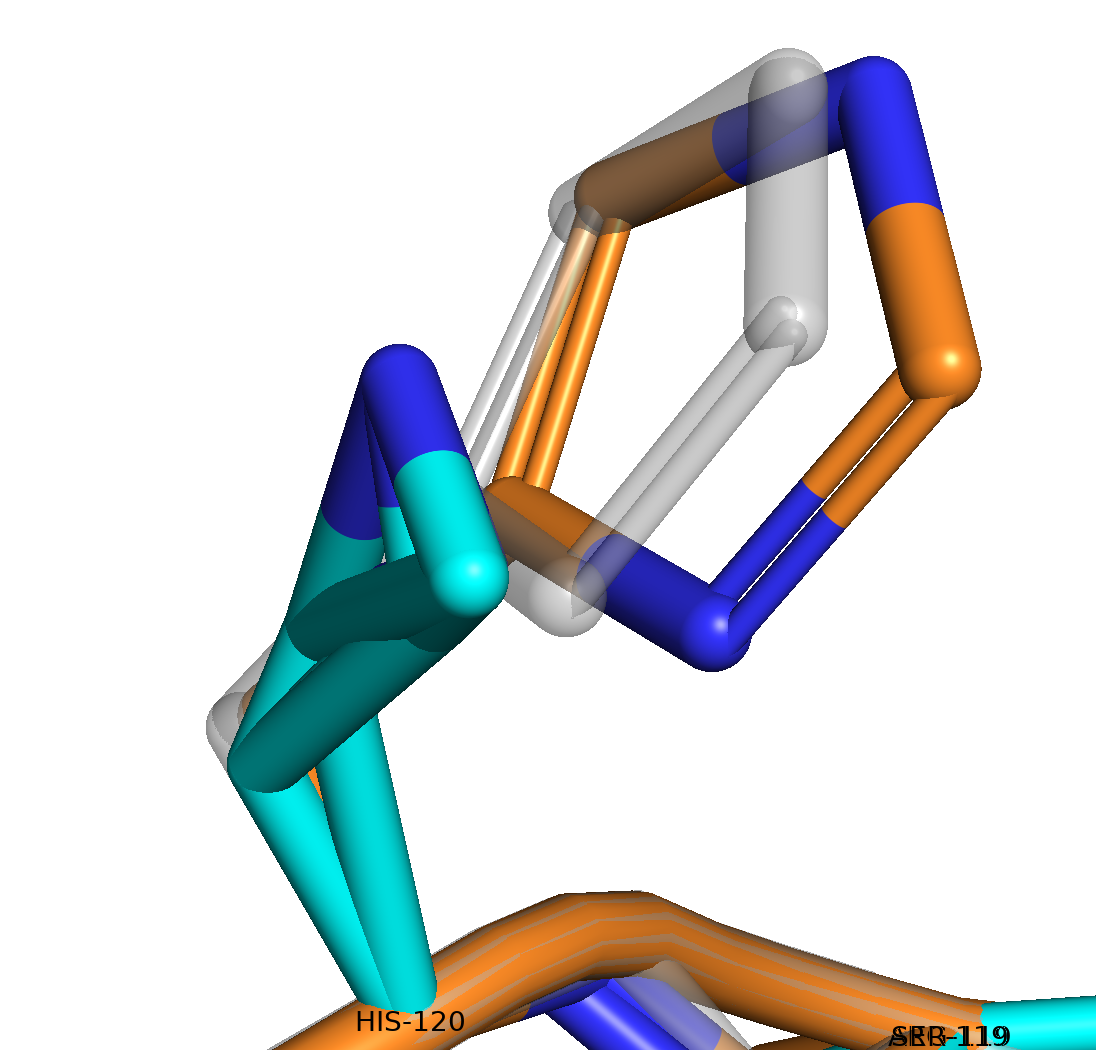
\includegraphics[width=\linewidth,height=55mm,keepaspectratio]{figures/results/failure-mode.png}
    \par\smallskip\textbf{(a)}
\end{minipage}\hfill
\begin{minipage}[t]{0.48\linewidth}
    \centering
    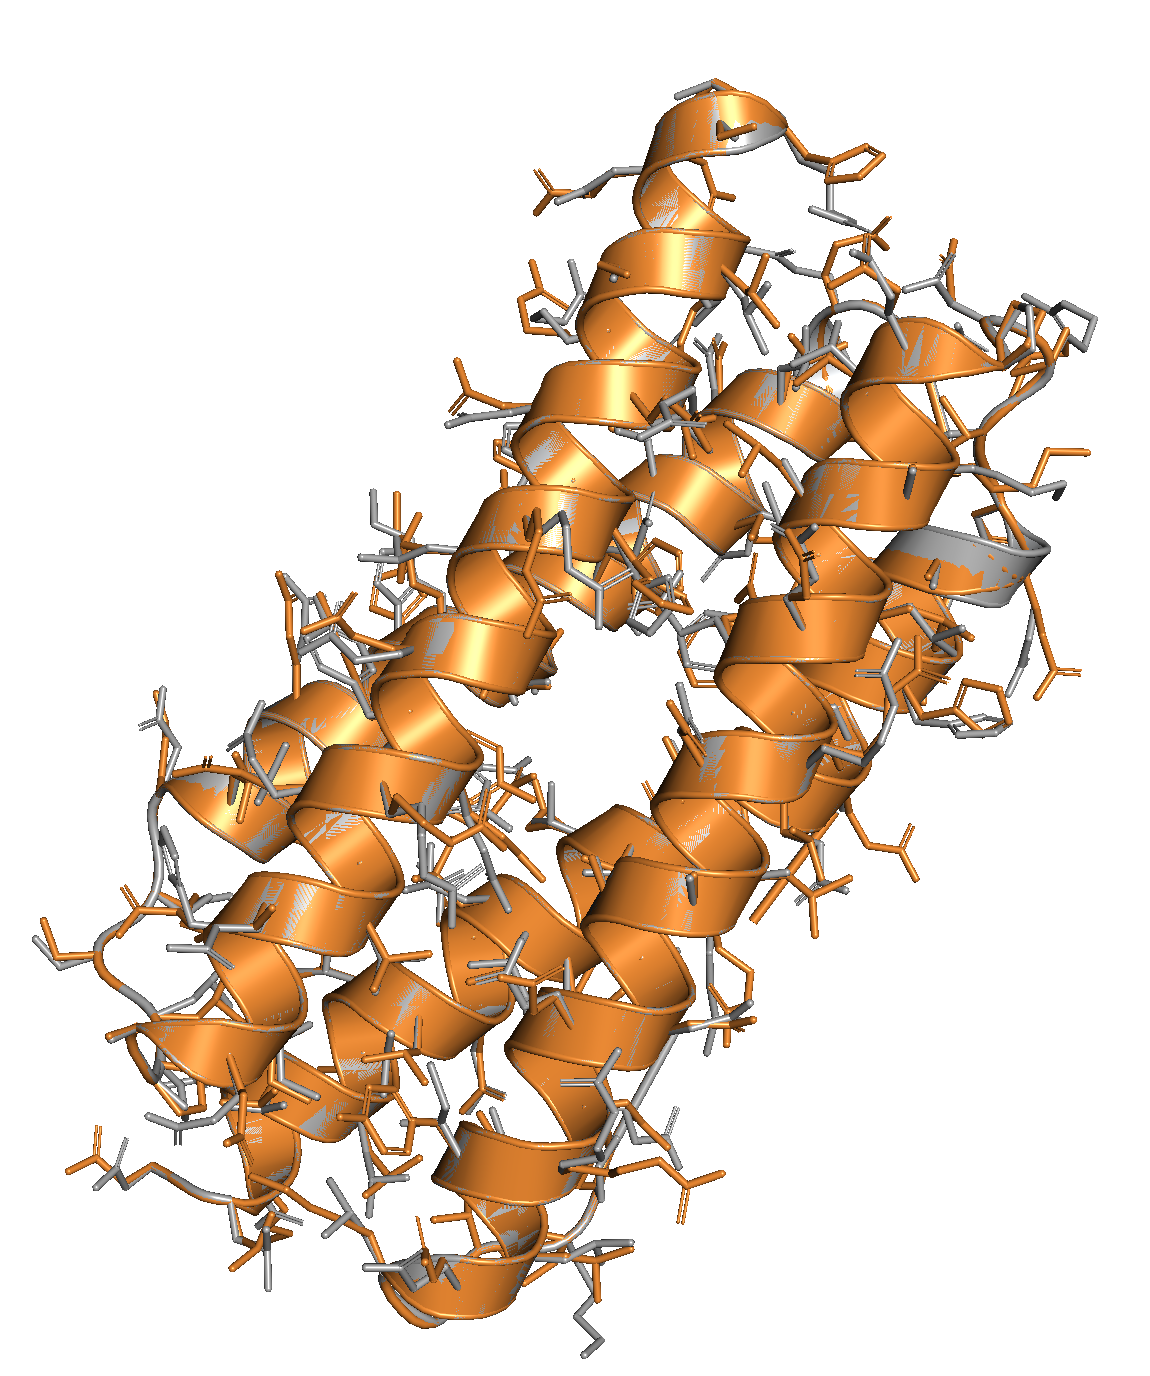
\includegraphics[width=\linewidth,height=55mm,keepaspectratio]{figures/results/reconst.png}
    \par\smallskip\textbf{(b)}
\end{minipage}
\caption{JEPA reconstruction examples. (a) HIS-120 in 5FLI chain A. The direct JEPA output (cyan) forms a chemically invalid local geometry, which is repaired by the postprocessing described in Section~\ref{sec:methods-reconstruction}. The native residue is transparent grey and the postprocessed reconstruction is orange. (b) Full-structure overlay for 4ETR chain A, with the native protein in grey and the postprocessed JEPA reconstruction in orange. Their backbones overlap closely, as expected from C$\alpha$ conditioning. Some side chains align well, while others retain angular or positional errors.}
\label{fig:reconstruction-postprocessed}
\end{figure}

\researchfindingbox{JEPA retains substantial sequence and structural information, but reconstructs atoms less accurately than the C$\alpha$ baseline.}

\subsection{Residue and Protein Organisation}
\label{sec:results-organisation}
\researchquestionbox{How do the latent spaces organise residue embeddings?}

\textbf{Linear probes.}
We evaluate amino-acid identity using two tests.
A linear classifier on the frozen embeddings predicts amino-acid identity with approximately 100\% accuracy for autoencoders, 69.3\% for random initialisation and 10.6\% for JEPA-70 (Table~\ref{tab:results-residue-probes}).
Amino-acid neighbour purity at $k=10$ is 100.0/99.9\% for the two autoencoders, 95.1\% for random initialisation, 45.1/45.3\% for absolute-position JEPA+SIGReg with 50/70\% masking and 21.7/23.0\% for JEPA with 50/70\% masking.
Thus, the autoencoders retain amino-acid identity almost perfectly, whereas uncropped LeJEPA shows the best secondary-structure (56.7\%). Relative-position JEPA+SIGReg with 50\% masking has the best RSA readout ($0.163$).
B-factor correlations are low across all models.

\par\bigskip\noindent
\begin{minipage}{\linewidth}
\centering
\setstretch{1}\fontsize{9.3}{11.1}\selectfont
\setlength{\tabcolsep}{4.3pt}
\begin{tabular}{lrrrr}
\toprule
Encoder & AA accuracy & SS accuracy & RSA $R^2$ & B-factor $\rho$ \\
\midrule
Random init. & 0.693 & 0.472 & 0.111 & 0.015 \\
$C_\alpha$ AE & 1.000 & 0.482 & 0.077 & 0.009 \\
Fully latent AE & 1.000 & 0.480 & 0.097 & 0.012 \\
JEPA 50 & 0.097 & 0.510 & 0.040 & 0.045 \\
JEPA 70 & 0.106 & 0.566 & 0.110 & 0.039 \\
JEPA mutation & 0.099 & 0.496 & 0.118 & 0.016 \\
JEPA+SIGReg 50 abs. & 0.097 & 0.476 & 0.007 & 0.069 \\
JEPA+SIGReg 70 abs. & 0.097 & 0.477 & 0.004 & 0.080 \\
JEPA+SIGReg mutation & 0.096 & 0.476 & 0.004 & 0.047 \\
JEPA+SIGReg 50 rel. & 0.097 & 0.482 & 0.163 & 0.036 \\
JEPA+SIGReg 70 rel. & 0.096 & 0.474 & 0.092 & 0.025 \\
LeJEPA, uncropped (EMA) & 0.099 & 0.567 & 0.029 & 0.014 \\
\bottomrule
\end{tabular}
\captionof{table}{Final-8D linear outputs for encoders at 100k and a random-init encoder, with probes for each case. AA = amino-acid identity. The uncropped LeJEPA row uses EMA weights.}
\label{tab:results-residue-probes}
\end{minipage}
\par\bigskip

Figure~\ref{fig:results-latent-organisation-100k} shows marked differences in latent-space organisation across selected models, with clearly separated amino-acid clusters in the autoencoder but more mixed identities in JEPA and LeJEPA.

\par\addvspace{1.5\baselineskip}\noindent
\begin{minipage}{\linewidth}
\centering
\makebox[\linewidth][c]{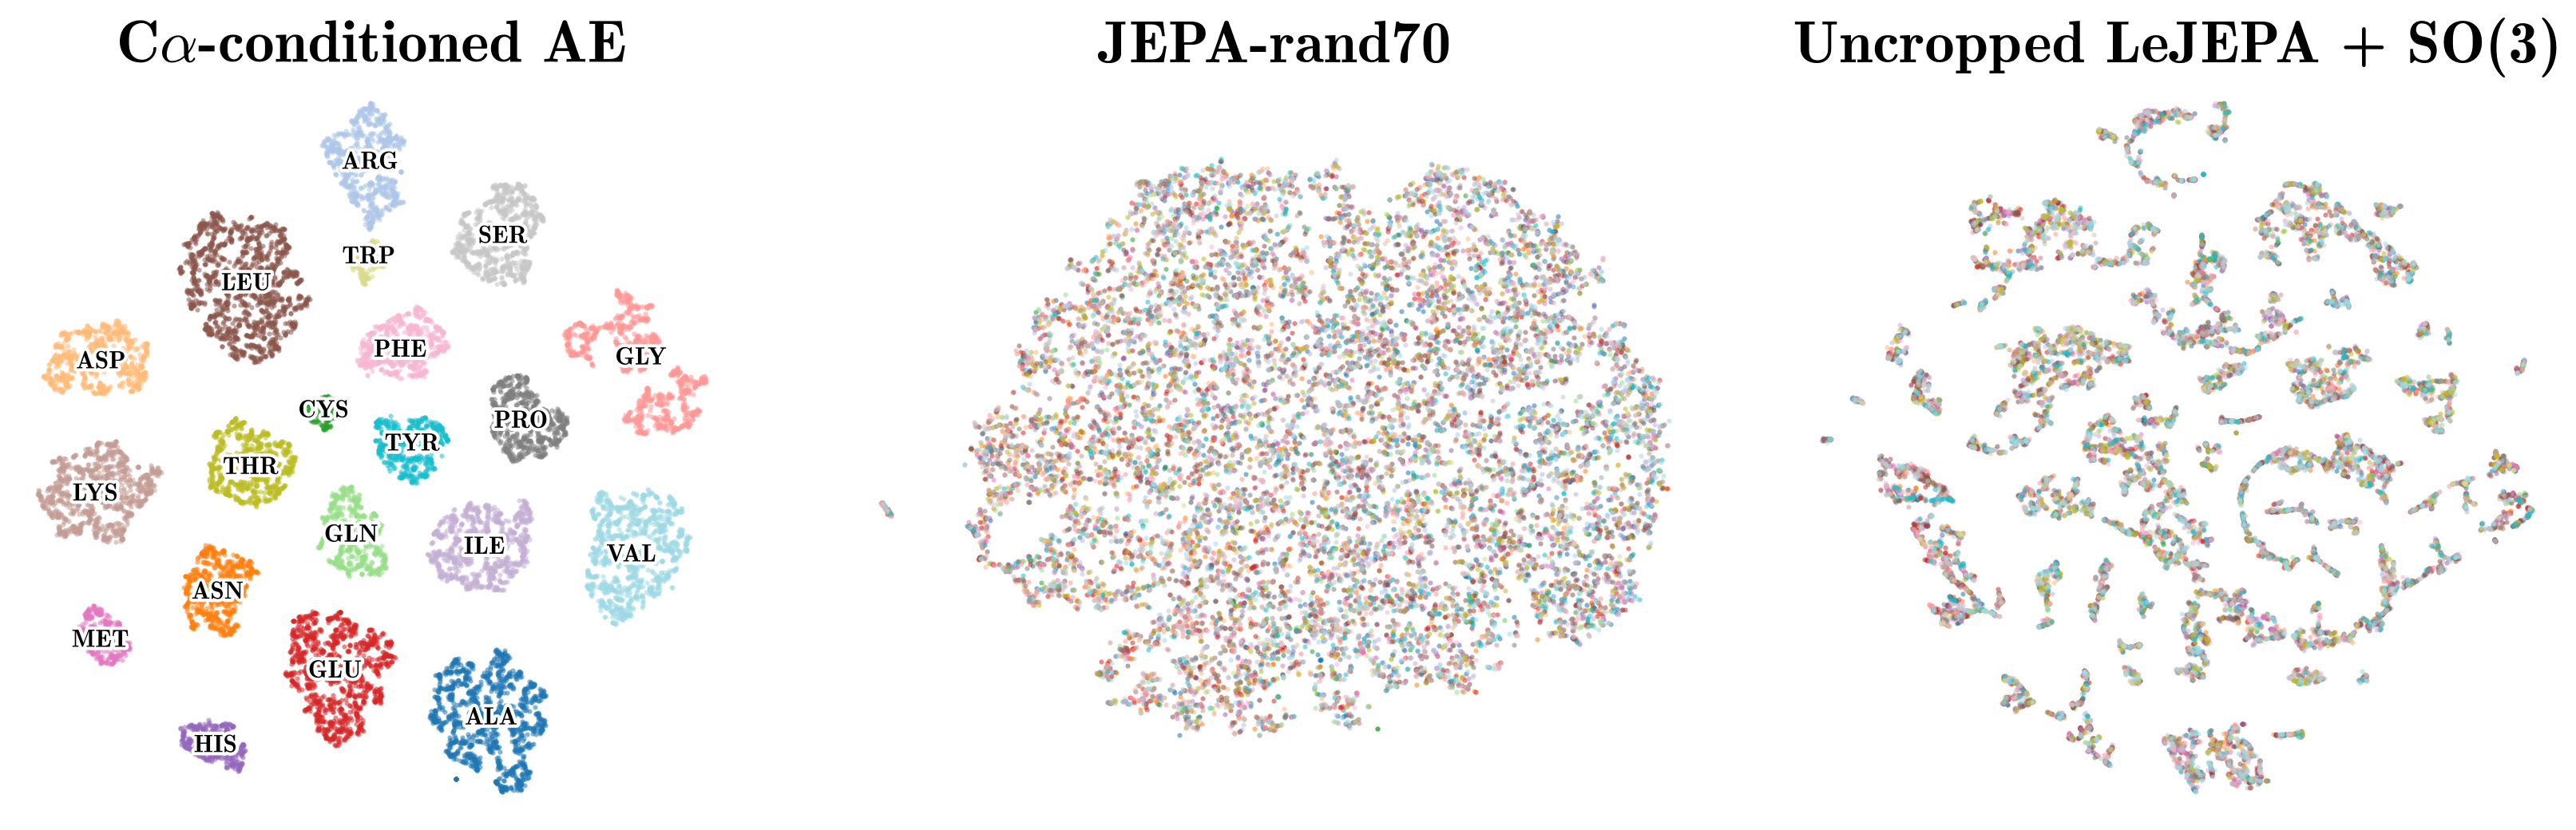
\includegraphics[width=1.04\linewidth]{figures/results/tsne_aa_ca_cond_jepa70_uncropped_lejepa_so3_100k.png}}
\captionof{figure}{t-SNE projections of residue embeddings from the C$\alpha$-conditioned autoencoder (left), JEPA with 70\% random masking (middle), and uncropped LeJEPA + SO(3) (right), at 100k checkpoints. Different colours represent different amino acids, labelled in the AE subfigure.}
\label{fig:results-latent-organisation-100k}
\end{minipage}
\par\addvspace{1.5\baselineskip}

\textbf{Absolute residue index.}
The downstream performance difference between absolute- and relative-position JEPA+SIGReg raises the question of how positional information influences the learned representations.
We use t-SNE to visualise which residues form similar neighbourhoods in latent space and whether these neighbourhoods reflect properties such as residue identity or position.
Figure~\ref{fig:results-index-100k} compares JEPA+SIGReg with 50\% random masking using absolute (left) and relative positions (right), with residues coloured by their absolute index within the chain.
Repeated strands are visible in the absolute-position latent space, and its local neighbourhoods are ordered by residue index.
This reveals a shortcut in which absolute position becomes a dominant feature of the representation.
Using relative target-context offsets removes this strand structure.

Relative positioning reduces exact-index purity at $k=10$ from 94.27\% to 1.61\%. The fraction of queries whose closest neighbour shares the same index falls from 97.25\% to 6.43\%.
Thus, the absolute-position result mostly reflects residues at matching indices across different proteins.

\begin{figure}[htbp]
\vspace{0.4\baselineskip}
\centering
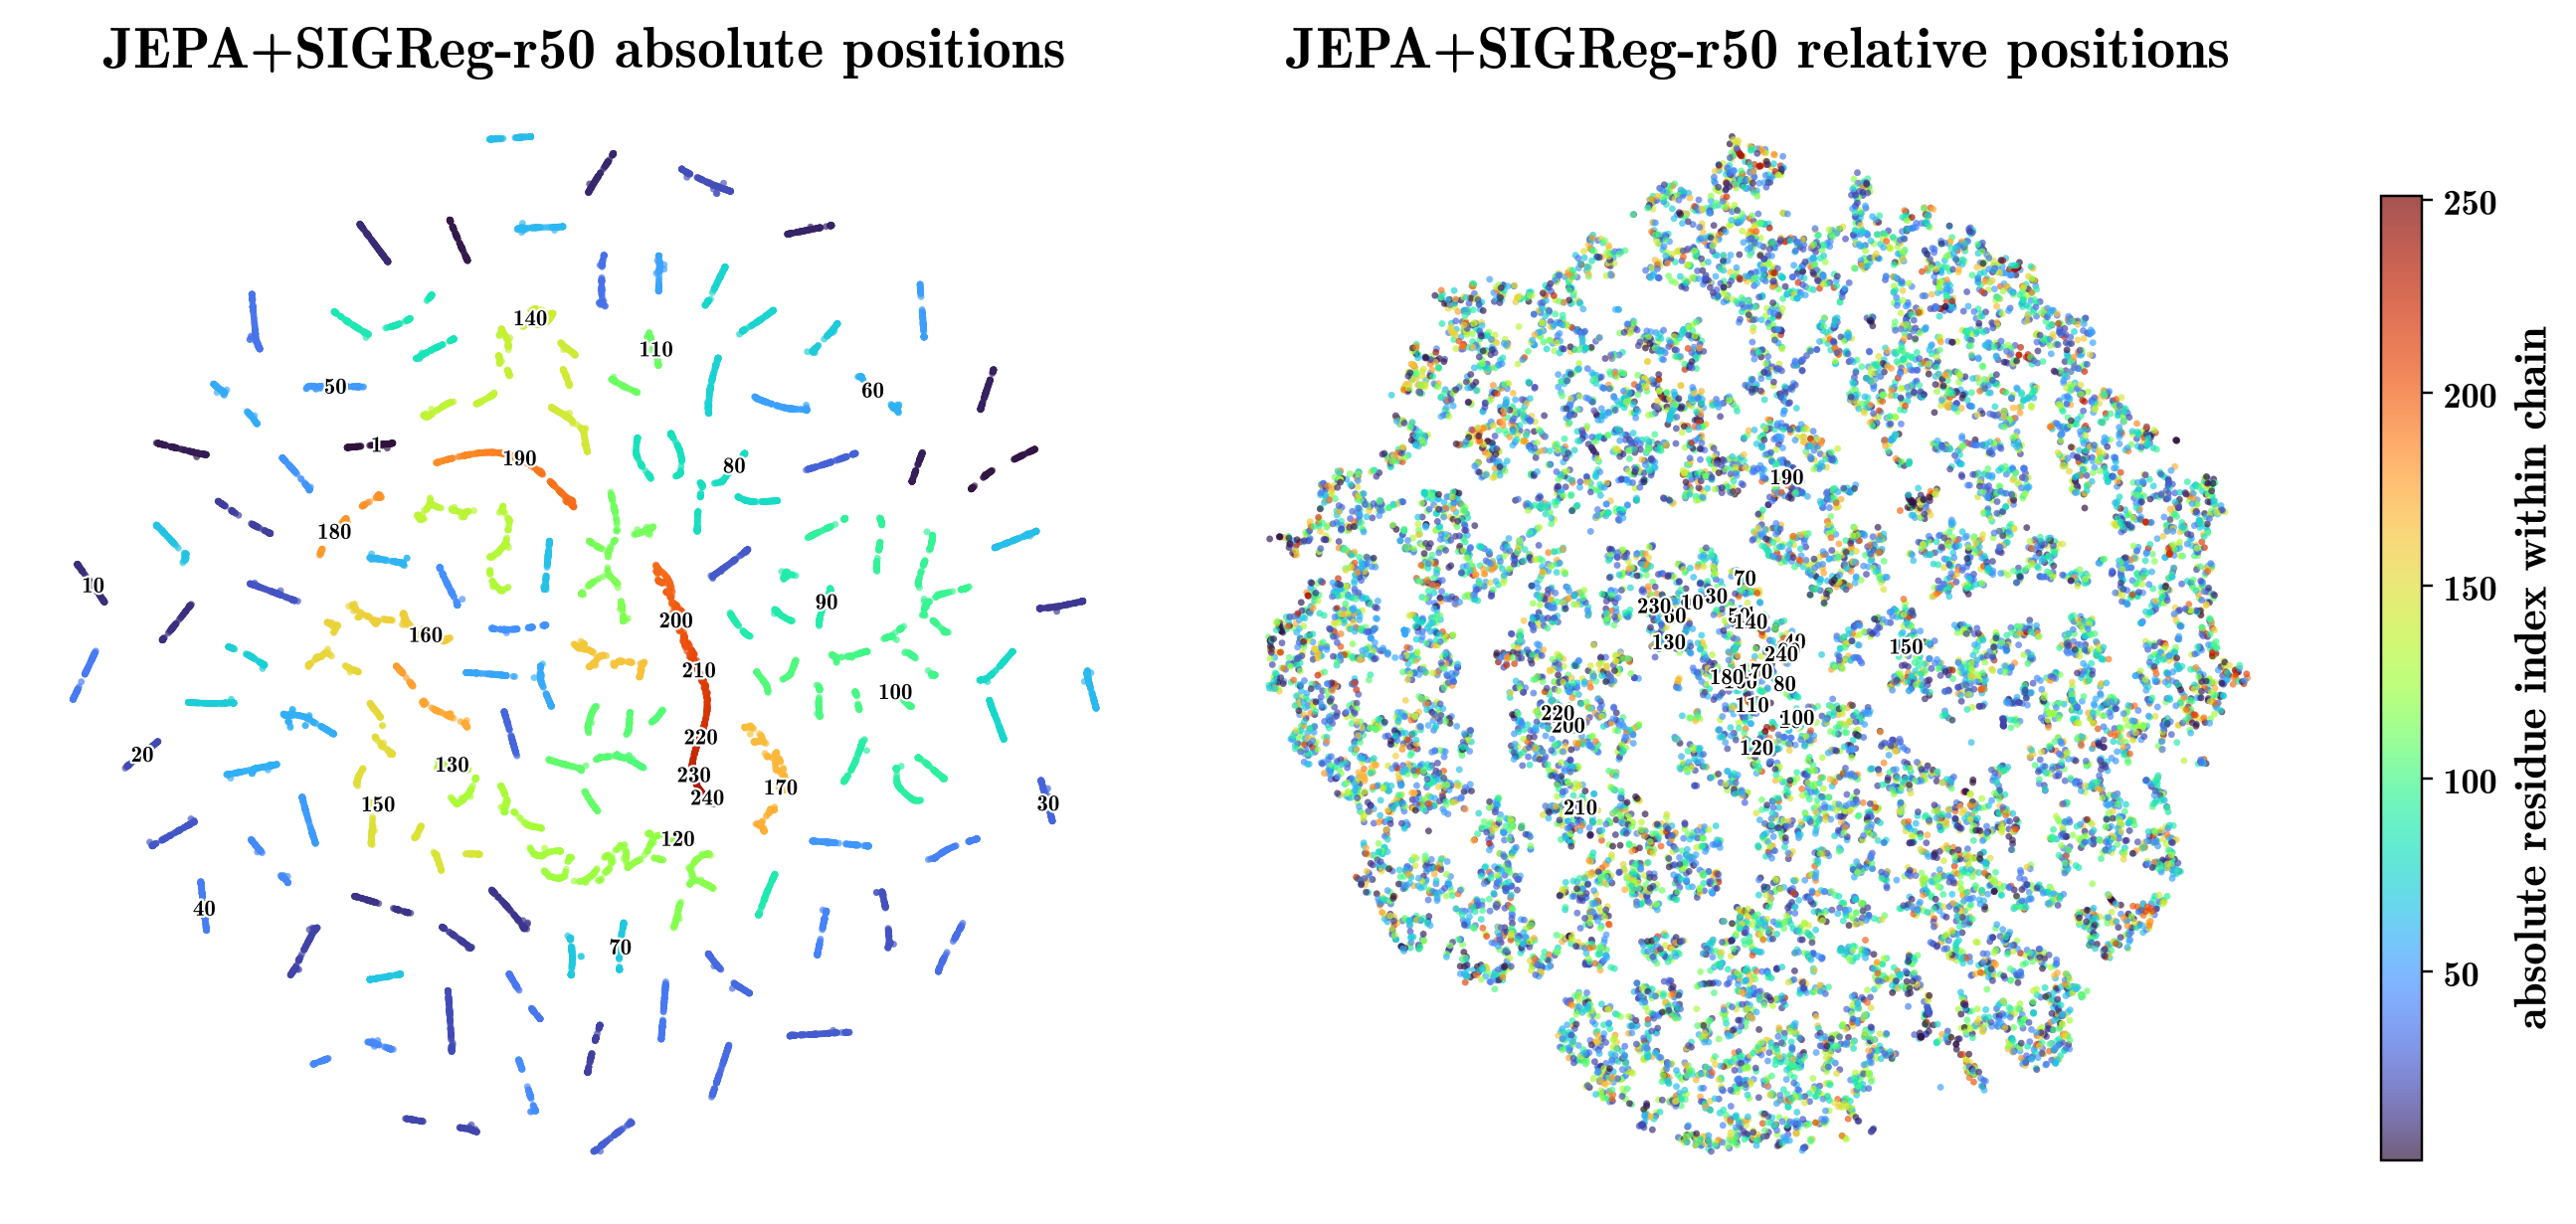
\includegraphics[width=\linewidth]{figures/results/tsne_lejepa-r50_absolute-v-relative_absolute-index_100k.png}
\caption{JEPA+SIGReg with 50\% random masking at 100k steps, using absolute positions (left) and relative positions (right). Numbers and colours on the strands indicate the absolute residue index within each chain, with an index range of [1-251].}
\label{fig:results-index-100k}
\vspace{0.4\baselineskip}
\end{figure}

Besides suppressing the residue-index shortcut, relative positioning also improves downstream performance.
For 70\% masking, it increases CatBio fold AUROC ($0.529$ to $0.733$) and FlexRMSF fold correlation ($0.108$ to $0.290$), and scores higher on 19/24 tasks. With 50\% masking, it improves on 18/24 tasks.
Although the relative-position model still receives pair features and signals from chain boundaries and length that can reveal approximate location, it removes the direct absolute target-position shortcut.


\textbf{Chain length.}
Uncropped LeJEPA also organises residues by chain length: residues from proteins of similar length form neighbourhoods in latent space (Figure~\ref{fig:results-chain-length-raw10k}).
In the cropped version, each crop has a fixed length, regardless of the protein's chain length.
To isolate the effect of cropping, we compare uncropped and cropped models while keeping every other setting unchanged, including 20\% global and 80\% local masking. Cropping reduces the chain-length correlation from $0.884$ to $0.193$, but effective rank also falls from $7.10$ to $1.61$. Retaining 80\% local masking means that only around ten visible residues remain in each 48-residue local crop, which appears too aggressive for the shorter view. We therefore use 50\% local masking in the reported cropped models, leaving around 24 visible residues and retaining near-full effective rank ($7.85/8$). The model also uses a larger batch, which, together with the lower masking rate, likely helps maintain this healthy rank.

\begin{figure}[htbp]
\vspace{0.4\baselineskip}
\centering
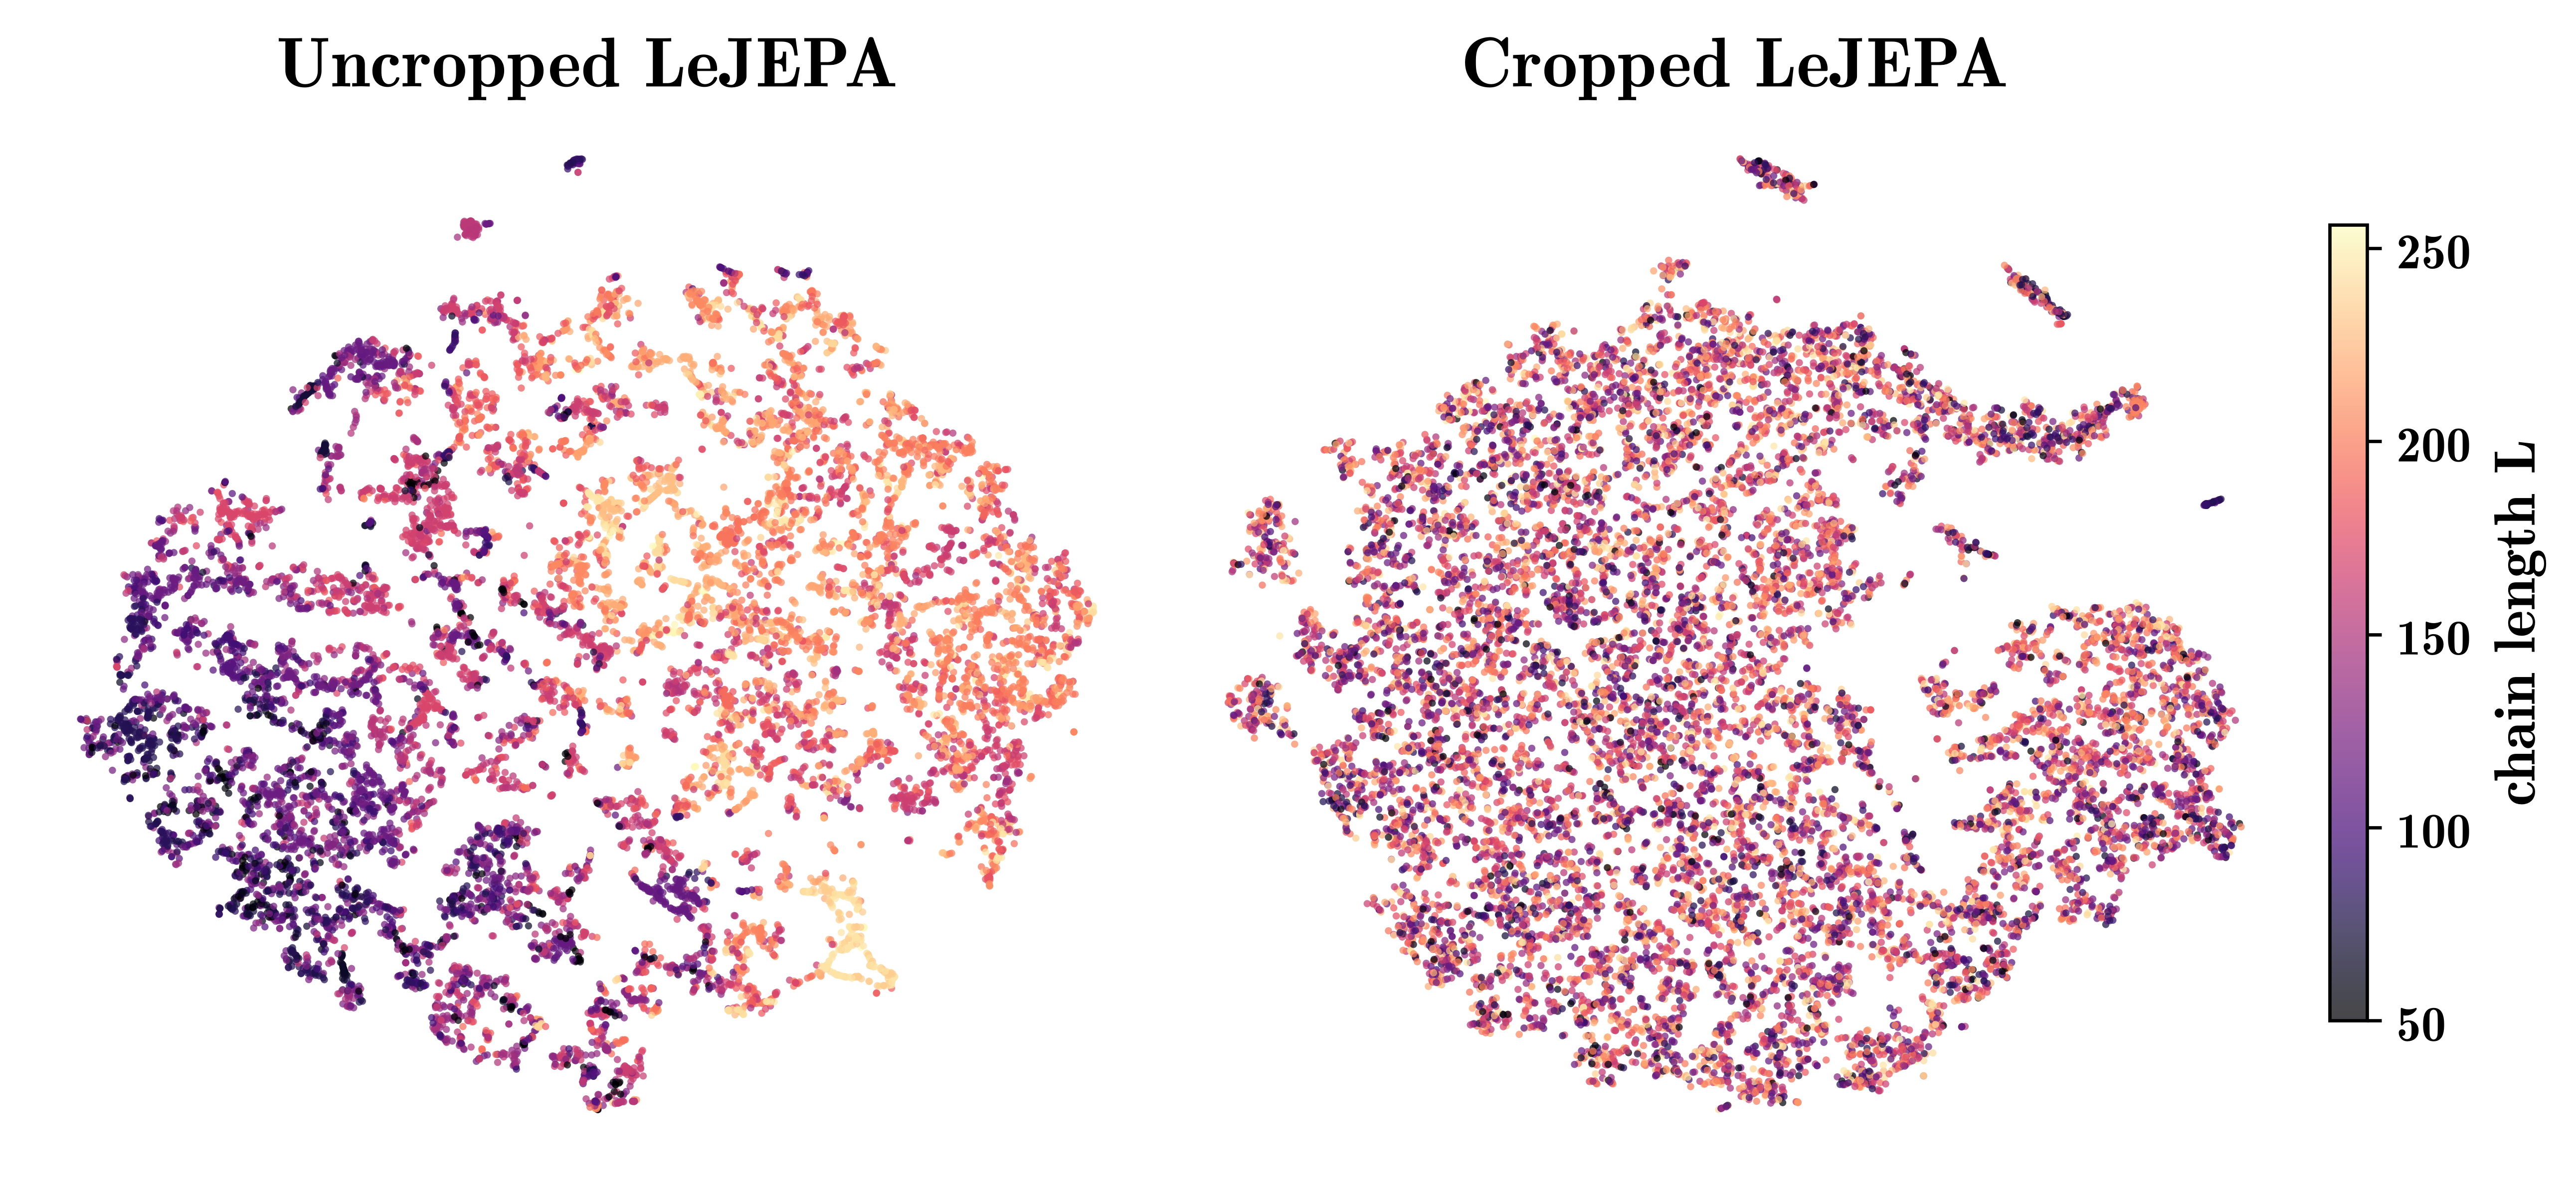
\includegraphics[width=0.95\linewidth]{figures/results/chain_length_tsne_matched_crop_control_raw10k.png}
\caption{Matched uncropped versus cropped LeJEPA comparison at the raw 10k checkpoint. Both models use mean-pooled protein views and differ only in cropping. Residue embeddings are coloured by chain length. Chain-length correlation decreases from $\rho=0.884$ to $0.193$, while effective rank decreases from $7.10$ to $1.61$.}
\label{fig:results-chain-length-raw10k}
\vspace{0.4\baselineskip}
\end{figure}

\textbf{Protein-level structural neighbourhoods.}
Across the four representations, nearest latent neighbours have mean TM-score gains of $0.216$-$0.456$ over the length-matched controls. However, their mean sequence identity is also higher ($0.404$-$0.689$ versus $0.151$). Below 30\% sequence identity, mean TM-score differences range from $-0.028$ to $0.015$, with every 95\% confidence interval including zero. The selected latent spaces therefore group homologous, structurally related proteins, but do not show structural organisation beyond sequence similarity.


\textbf{Independent rotations.}
\label{sec:results-rotation-64d}
Figure~\ref{fig:results-rotation-64d-60k} compares 64D JEPA with 70\% random residue masking, without and with independently rotated context and target views at 60k.
The model trained with rotated views forms clearer amino-acid clusters.
A 10k checkpoint rotation ablation in Appendix~\ref{app:latent-figures} shows that the same trend is present early on. However, a matched latent-width control shows that rotations alone are insufficient: with rotations in both models, the 64D representation forms amino-acid clusters whereas the 8D representation does not. Amino-acid neighbour purity falls from $0.974$ to $0.109$, suggesting that the 8D bottleneck discards much of the residue-identity information retained in 64D. Thus, the clustering reflects an interaction between rotation augmentation and latent capacity rather than rotations alone. These plots show changes in representation organisation, but do not establish rotation invariance.

\begin{figure}[htbp]
\centering
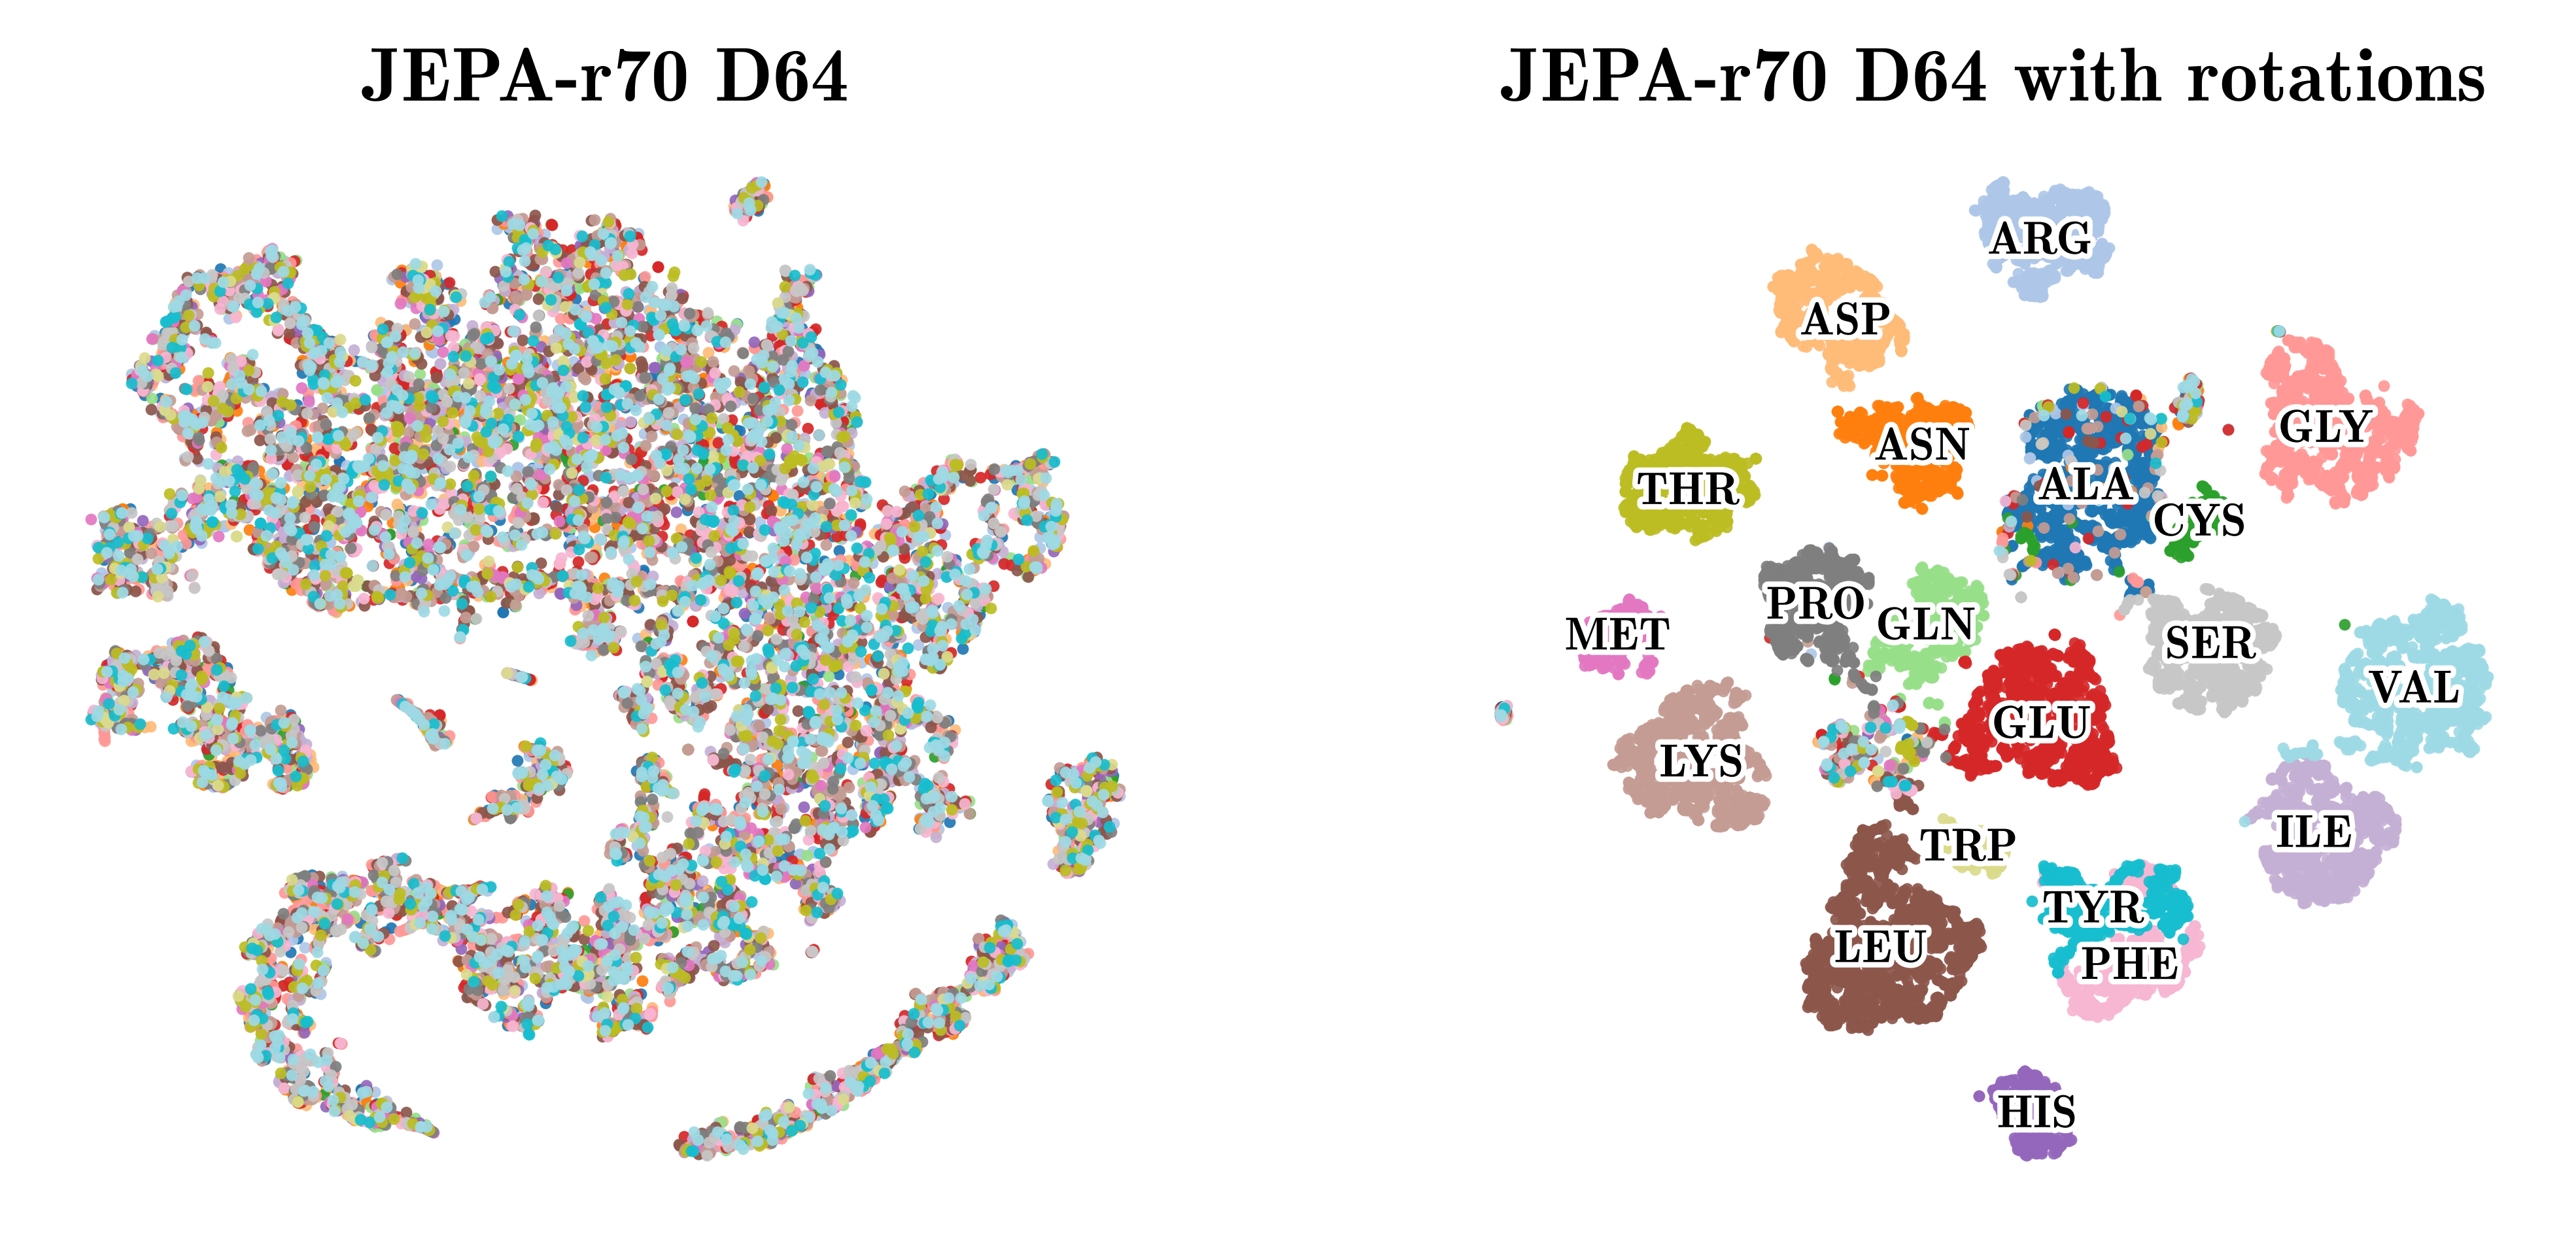
\includegraphics[width=0.88\linewidth]{figures/results/tsne_aa20_jepa-r70-d64-60k-v-rotation-60k_labels-on-clusters.png}
\caption{64D JEPA rotation comparison at 60k with 70\% random masking, without (left) and with (right) independent SO(3) view rotations. Different colours represent different amino acids, labelled in the rotated-view model.}
\label{fig:results-rotation-64d-60k}
\end{figure}
\researchfindingbox{Positional and geometric design choices strongly shape what information the learned representations retain. Relative positioning reduces absolute-index organisation and improves most downstream task scores, while independent rotation augmentation can produce clearer amino-acid clusters.}

\subsection{Rotation Invariance and Effective Rank}
\label{sec:results-collapse}

We monitor effective rank as a representation-health diagnostic and to detect collapse. For these 8D representations, a rank near one can indicate that most variation has collapsed into a single direction, whereas a higher rank can indicate healthier use of the latent space. However, higher rank does not necessarily guarantee better downstream performance.

Table~\ref{tab:results-rank-stb-10k} compares uncropped LeJEPA with and without independent SO(3) view rotations, retaining the same masking and objective settings. The rotated model has lower effective rank ($3.22$ versus $7.17$), yet scores higher on 21/24 tasks. The table shows four of these improvements. We suspected that this difference might be related to the effect of rotation augmentation rather than simple representation collapse. Our hypothesis was that learning from diverse rotated views removes orientation-dependent variation and concentrates the remaining information into fewer dimensions.

Therefore, we test rotation invariance. Across 400 chains (59,750 residues) and 16 rotations per chain, corresponding residue latents have mean protein-centred cosine similarity $0.765\;[0.756,0.774]$ with rotation training and $0.277\;[0.269,0.285]$ without it (95\% CIs). The increase occurs for every sampled protein, while randomly mismatched residues have similarities near zero. This supports our hypothesis and could explain the rotated model's lower effective rank. Further analysis is needed to determine what each latent dimension directly encodes.

\begin{table}[htbp]
\centering
\resultstableformat
\fontsize{9}{10.8}\selectfont
\setlength{\tabcolsep}{4pt}
\begin{tabular}{@{}lrrrrr@{}}
\toprule
Model & Rank /8 & \shortstack{BindShake\\AUROC} & \shortstack{CatBio fold\\AUROC} & \shortstack{FlexRMSF fold\\$\rho$} & \shortstack{Homo family\\macro-F1} \\
\midrule
Uncropped LeJEPA & 7.17 & 0.639 & 0.595 & 0.337 & 0.093 \\
Uncropped LeJEPA+SO(3) & 3.22 & \textbf{0.769} & \textbf{0.733} & \textbf{0.532} & \textbf{0.196} \\
\bottomrule
\end{tabular}
\caption{Uncropped LeJEPA at 10k (EMA weights) with and without rotations. SIGReg weight $0.02$ in both runs. Task scores use L600 STB evaluation.}
\label{tab:results-rank-stb-10k}
\end{table}

\subsection{Layerwise Information and the Latent Bottleneck}
\label{sec:results-layerwise}
\researchquestionbox{Is the final 8D latent the most useful representation for downstream tasks?}

Here, we examine encoder blocks 1, 6 and 12 and the final 8D latent mean of uncropped LeJEPA without rotations at 100k, starting from the model output and moving backwards through the encoder. Block 12 scores higher than the final 8D latent on 20/24 STB task scores, showing that more downstream-accessible information is available before the final projection.
Moving earlier in the encoder, block 6 scores higher than block 12 on 22/24 tasks and has the highest score among all four representations on 19/24. Both block outputs are 768-dimensional, so this comparison keeps the representation width fixed. Compared with the final 8D latent, BindShake AUROC increases from $0.585$ to $0.831$, FlexRMSF fold correlation from $0.225$ to $0.634$, and all six flexibility scores are higher.

Block 6 also exceeds the best final-8D score among the 18 models in main Table~\ref{tab:results-stb-main} on 22 of 24 task/split scores. The exceptions are Rep fold and Ept fold.
The largest gains are in flexibility: FlexRMSF fold ($0.634$ vs.\ $0.428$) and FlexNEQ fold ($0.514$ vs.\ $0.251$).
The progression is not monotonic: block 1 is strongest on BindBio fold and CatBio superfamily, block 12 on Con fold, and the final mean on Rep fold and Ept fold.
The random-init block-6 control is highest only on Rep fold, showing that the 768D input alone does not account for the improvements.

The same pattern appears in JEPA with 70\% random masking, where block 6 outperforms the final 8D latent on all nine evaluated task scores (Appendix~\ref{app:jepa-r70-layerwise}). Layerwise linear probes provide complementary evidence, with higher AA and SS accuracy in earlier blocks than in the final 8D latent (Appendix~\ref{app:layerwise-supporting}, Figure~\ref{fig:results-layer-probes}).

{\textbf{Encoder with six blocks.} Finally, we trained uncropped LeJEPA without rotations using six encoder blocks instead of twelve.
At 100k, its final 8D mean improves 15/24 scores over the 12-block model's final 8D mean, including all six flexibility scores (Appendix~\ref{app:encoder-depth}, Table~\ref{tab:results-encoder-depth}).
However, it remains below the original twelve-block encoder's intermediate block 6 on 23 of 24 scores. Thus, reducing encoder depth alone does not recover that performance.}

\researchfindingbox{Block 6 provides a more useful representation for most downstream tasks, exceeding the best final-8D score across all 18 main Table~\ref{tab:results-stb-main} entries on 22/24 task scores.}

\clearpage

\begin{table}[p]
\centering
\resultstableformat
\setlength{\tabcolsep}{1.8pt}
\renewcommand{\arraystretch}{0.86}
\caption{Full-L600 STB for uncropped LeJEPA without rotations at 100k, using raw weights and full-context evaluation. Scores are multiplied by 100. Higher is better, and row maxima are bold. The first four model columns are readouts from the 12-block encoder. Random-init block 6 is an untrained 768D control. The 768D and 8D readouts give the downstream head different input parameterisations. The final column gives the percentage change from the final 8D score to block 6. Large percentages arise when final-8D scores are near zero.}
\label{tab:results-layer-stb}
\sbox{\stbpreviewbox}{%
\begin{tabular}{@{}lllrrrrrr@{}}
\toprule
\multirow{2}{*}{Task type} & \multirow{2}{*}{Task} & \multirow{2}{*}{Split} & \multicolumn{4}{c}{12-block uncropped LeJEPA} & \multicolumn{1}{c}{Control} & \multicolumn{1}{c}{Change} \\[1.8pt]
& & & \shortstack{Block 1\\768D} & \shortstack{Block 6\\768D} & \shortstack{Block 12\\768D} & \shortstack{Final mean\\8D} & \shortstack{Random init.\\block 6, 768D} & \shortstack{$\Delta$ vs.\\final 8D (\%)} \\
\midrule
\multicolumn{9}{c}{\textbf{Functional-site prediction: AUROC $\times100$}} \\
\midrule
\multirow{5}{*}{Binding site}
& \multirow{2}{*}{BindInt} & Fold & 46.49 & \textbf{52.19} & 46.68 & 50.30 & 48.98 & +3.8 \\
& & SF & 93.16 & \textbf{94.13} & 90.96 & 88.45 & 88.06 & +6.4 \\
& \multirow{2}{*}{BindBio} & Fold & \textbf{78.35} & 78.31 & 71.32 & 59.32 & 74.12 & +32.0 \\
& & SF & 79.30 & \textbf{80.04} & 71.18 & 61.82 & 74.58 & +29.5 \\
& BindShake & Test & 79.61 & \textbf{83.11} & 80.38 & 58.45 & 78.23 & +42.2 \\
\multirow{4}{*}{Catalytic site}
& \multirow{2}{*}{CatInt} & Fold & 67.23 & \textbf{69.36} & 57.25 & 51.71 & 64.32 & +34.1 \\
& & SF & 94.48 & \textbf{95.78} & 88.98 & 80.74 & 88.95 & +18.6 \\
& \multirow{2}{*}{CatBio} & Fold & 83.27 & \textbf{85.05} & 80.17 & 53.67 & 81.87 & +58.5 \\
& & SF & \textbf{94.40} & 94.04 & 82.98 & 60.61 & 91.41 & +55.2 \\
\multirow{2}{*}{Conserved site}
& \multirow{2}{*}{Con} & Fold & 68.07 & 68.22 & \textbf{72.61} & 60.10 & 63.47 & +13.5 \\
& & SF & 88.83 & \textbf{92.16} & 84.21 & 77.27 & 81.40 & +19.3 \\
\multirow{2}{*}{Repeat motif}
& \multirow{2}{*}{Rep} & Fold & 67.95 & 60.39 & 53.50 & 71.05 & \textbf{76.66} & -15.0 \\
& & SF & 85.40 & \textbf{91.66} & 80.96 & 83.49 & 79.48 & +9.8 \\
\multirow{2}{*}{Epitope region}
& \multirow{2}{*}{Ept} & Fold & 55.58 & 55.70 & 61.36 & \textbf{62.00} & 55.61 & -10.2 \\
& & SF & 69.33 & \textbf{76.09} & 65.93 & 59.72 & 69.06 & +27.4 \\
\midrule
\multicolumn{9}{c}{\textbf{Remote homology: macro-F1 $\times100$}} \\
\midrule
\multirow{3}{*}{Remote homology}
& \multirow{3}{*}{Homo} & Fold & 14.56 & \textbf{16.94} & 9.68 & 6.73 & 6.64 & +151.7 \\
& & Family & 36.89 & \textbf{39.88} & 26.89 & 19.64 & 21.76 & +103.1 \\
& & SF & 17.19 & \textbf{19.90} & 8.52 & 5.54 & 6.77 & +259.2 \\
\midrule
\multicolumn{9}{c}{\textbf{Structural flexibility: Spearman's $\rho\times100$}} \\
\midrule
\multirow{6}{*}{Flexibility}
& \multirow{2}{*}{FlexRMSF} & Fold & 52.41 & \textbf{63.39} & 42.74 & 22.48 & 43.84 & +182.0 \\
& & SF & 53.13 & \textbf{68.52} & 52.51 & 30.96 & 41.73 & +121.3 \\
& \multirow{2}{*}{FlexBFactor} & Fold & 34.28 & \textbf{37.71} & 22.56 & 5.01 & 31.14 & +652.7 \\
& & SF & 29.65 & \textbf{32.73} & 20.58 & 3.50 & 27.15 & +835.1 \\
& \multirow{2}{*}{FlexNEQ} & Fold & 46.97 & \textbf{51.39} & 39.73 & 2.46 & 19.11 & +1989.0 \\
& & SF & 46.70 & \textbf{50.69} & 39.76 & 3.54 & 19.29 & +1331.9 \\
\bottomrule
\end{tabular}%
}
\stbpreviewfit
\end{table}
\clearpage

\subsection{Discussion}
\label{sec:results-discussion}

This discussion connects the downstream, latent-space, reconstruction and layerwise results, interpreting what the models retain and where the objectives introduce trade-offs or shortcuts. We examine how the objective and design choices shape which information remains accessible.

\subsubsection{Predictive Objectives and Downstream Transfer}

The central question of this thesis is whether predicting or aligning latent representations can capture information useful for protein structure and function. The results support this idea, but no model is uniformly strongest. Because StructTokenBench spans residue- and protein-level properties, the task-specific results show that information useful at one biological scale is not automatically strongest at another. Together with the differences in latent-space organisation, this suggests that the objective and view construction shape which information remains accessible rather than making a representation uniformly better or worse.
Mutation conditioning extends this question to interventions (Section~\ref{sec:results-mutation}). Its downstream changes remain difficult to isolate because the action input, mutant target and training loss change together. It should therefore be interpreted as a first implementation of mutation actions rather than a complete mutation model.

\subsubsection{Masking and Shortcut Learning}

The benefit of 70\% random masking in JEPA is consistent with I-JEPA's finding that sufficiently informative targets are important for latent prediction \citep{assran2023ijepa}. Masking changes both task difficulty and the shortcuts available to solve it, so harder prediction helps only when the model must use meaningful context. With learned absolute target positions, JEPA+SIGReg can organise its latent space almost directly by residue index. Relative offsets retain sequence separation while removing this direct identifier, and the simultaneous reduction in index purity and improvement in downstream scores indicates that the shortcut had displaced more useful information. In LeJEPA, complete protein views expose the same chain length across views, whereas fixed-length crops reduce that organisation. The matched crop experiment also shows why only removing shortcuts is not enough. Chain-length correlation falls, but effective rank also falls to $1.61/8$, indicating that most variation is concentrated in very few directions (Section~\ref{sec:results-organisation}). A protein-specific view must therefore remove easy global or local shortcuts without making the remaining prediction problem uninformative or excessively difficult.

\subsubsection{Invariance and Representation Collapse}

Because protein properties should not depend on global orientation, we expected independent rotations to improve the learned representations more broadly. Rotations make corresponding residue embeddings substantially more consistent under changes in global orientation, but their downstream effect remains task- and model-dependent (Section~\ref{sec:results-collapse}). Similarly, SIGReg is necessary to prevent near-constant branches in JEPA+SIGReg, yet a near-full effective rank does not guarantee useful transfer. Rotated LeJEPA shows that the opposite can also occur, as fewer dominant directions coexist with stronger performance on most evaluated tasks. Thus, invariance and effective rank describe properties of a representation rather than its overall quality. Effective rank is best interpreted as a warning signal for dimensional collapse, alongside downstream and property-specific evaluations, rather than an objective we should maximise.

\subsubsection{Reconstruction Quality}

The reconstruction gap is expected because JEPA predicts latent representations and training never optimises the encoder for atom-level reconstruction. Reconstruction therefore tests how much atomic detail remains accessible, rather than whether JEPA can match an autoencoder trained for this task. The C$\alpha$ TM-score is 1.0 for all outputs because those coordinates are provided directly, so it cannot establish that JEPA recovers the global fold. The common-atom lDDT is higher than the true-sequence lDDT because sequence errors exclude some poorly reconstructed side-chain atoms from the common-atom metric. One possible explanation for the chemically invalid decoder geometries is that the coordinate and sequence losses do not explicitly enforce valid bond lengths, bond angles or separation between atoms. When several side-chain placements are possible, coordinate optimisation can also favour an average that is not a valid geometry. Postprocessing makes the structures more realistic, but its worse side-chain reconstruction metrics show that it can move atoms away from their native positions. Postprocessing is therefore useful for visualisation, without necessarily improving reconstruction.

\subsubsection{Intermediate Encoder Representations}

The block 12 result suggests that the final projection may discard downstream-accessible information, but it cannot separate the effect of the projection from the reduction to eight dimensions. The block 6 comparison is more direct because blocks 6 and 12 have the same width. Its stronger scores suggest that useful downstream features peak earlier in the encoder and may later become specialised or compressed. This does not mean that six encoder blocks are sufficient, since training a separate six-block model does not reproduce the intermediate output. Previous work similarly finds that intermediate representations can outperform final layers and explains this through the balance between preserving information and compressing it for the training objective \citep{skean2025layer}. Other protein language model studies also find that the best layer depends on the downstream task, and that many tasks reuse features learned before the final layer \citep{li2024featurereuse,joeres2026taskdataset}. Even with the dimensionality confound, these results highlight the importance of choosing which encoder layer to evaluate and place our structural encoder within the same broader pattern of useful intermediate representations (Section~\ref{sec:results-layerwise}).

\clearpage

\clearpage
\endinput
%TC:ignore
\appendix
\section{Downstream Results for Proteins up to 256 Residues}
\label{app:l256}
Table~\ref{tab:results-stb-l256} reports StructTokenBench results for proteins with at most 256 residues.
\begingroup
\ifdefined\stbworkshopbox\else\newsavebox{\stbworkshopbox}\fi
\providecommand{\stbworkshopfit}{\ifdim\wd\stbworkshopbox>\linewidth\resizebox{\linewidth}{!}{\usebox{\stbworkshopbox}}\else\usebox{\stbworkshopbox}\fi}
\begin{table}[p]
\centering
\resultstableformat
\setlength{\tabcolsep}{2pt}
\renewcommand{\arraystretch}{0.88}
\fontsize{7.5}{9}\selectfont
\caption{StructTokenBench evaluation restricted to proteins with at most 256 residues.}
\label{tab:results-stb-l256}
\sbox{\stbworkshopbox}{%
\begin{tabular}{@{}lllrrrrrrrr@{}}
\toprule
\multirow{2}{*}{Task type} & \multirow{2}{*}{Task} & \multirow{2}{*}{Split} & \multicolumn{2}{c}{Autoencoders} & \multicolumn{3}{c}{JEPA} & \multicolumn{3}{c}{JEPA+SIGReg} \\[1.8pt]
 & & & $C_\alpha$ & Full AE & 50\% & 70\% & Mut. & 50\% & 70\% & Mut. \\
\midrule
\multicolumn{11}{c}{\textbf{Functional-site prediction: AUROC $\times100$}} \\
\midrule
\multirow{5}{*}{Binding site} & \multirow{2}{*}{BindInt} & Fold & 41.69 & 40.66 & 40.54 & 42.03 & \textbf{42.14} & 38.91 & 40.65 & 39.69 \\
 &  & SF & 86.84 & 85.80 & 87.39 & 86.07 & 86.82 & \textbf{89.52} & 83.70 & 88.85 \\
 & \multirow{2}{*}{BindBio} & Fold & 62.96 & \textbf{65.32} & 55.60 & 58.54 & 57.47 & 57.12 & 57.47 & 57.16 \\
 &  & SF & 63.23 & \textbf{65.63} & 58.22 & 60.02 & 59.49 & 59.60 & 59.79 & 59.73 \\
 & BindShake & Test & 59.19 & \textbf{65.11} & 53.76 & 64.42 & 63.89 & 59.73 & 59.96 & 60.83 \\
\multirow{4}{*}{Catalytic site} & \multirow{2}{*}{CatInt} & Fold & 58.97 & \textbf{61.19} & 58.92 & 58.09 & 59.94 & 59.38 & 58.19 & 57.39 \\
 &  & SF & 76.50 & \textbf{76.82} & 73.79 & 75.37 & 75.36 & 74.33 & 75.91 & 76.47 \\
 & \multirow{2}{*}{CatBio} & Fold & 64.01 & \textbf{71.89} & 54.46 & 62.41 & 60.40 & 53.05 & 51.54 & 51.53 \\
 &  & SF & 78.31 & \textbf{84.44} & 65.48 & 71.96 & 69.87 & 62.06 & 61.68 & 63.21 \\
\multirow{2}{*}{Conserved site} & \multirow{2}{*}{Con} & Fold & 57.20 & \textbf{59.98} & 59.51 & 58.51 & 59.34 & 58.85 & 59.43 & 59.22 \\
 &  & SF & 71.97 & 73.48 & 70.73 & 71.22 & 72.43 & \textbf{74.30} & 74.10 & 74.11 \\
\multirow{2}{*}{Repeat motif} & \multirow{2}{*}{Rep} & Fold & 65.38 & 64.43 & 66.08 & 65.91 & 65.37 & \textbf{67.73} & 66.97 & 67.08 \\
 &  & SF & 80.79 & 79.82 & \textbf{82.00} & 79.24 & 81.25 & 77.65 & 76.02 & 77.46 \\
\multirow{2}{*}{Epitope region} & \multirow{2}{*}{Ept} & Fold & 56.28 & 55.21 & \textbf{59.29} & 54.79 & 56.57 & 58.34 & 56.67 & 55.90 \\
 &  & SF & 64.15 & 62.59 & \textbf{65.09} & 60.61 & 61.86 & 61.02 & 60.76 & 57.63 \\
\midrule
\multicolumn{11}{c}{\textbf{Remote homology: macro-F1 $\times100$}} \\
\midrule
\multirow{3}{*}{Remote homology} & \multirow{3}{*}{Homo} & Fold & 7.89 & 6.29 & 7.10 & \textbf{10.21} & 8.77 & 7.43 & 7.98 & 8.54 \\
 &  & Family & \textbf{35.26} & 26.86 & 17.67 & 21.29 & 17.00 & 21.52 & 20.01 & 26.60 \\
 &  & SF & 8.41 & 10.47 & 4.97 & \textbf{11.59} & 8.51 & 7.73 & 6.67 & 6.14 \\
\midrule
\multicolumn{11}{c}{\textbf{Structural flexibility: Spearman's $\rho\times100$}} \\
\midrule
\multirow{6}{*}{Flexibility} & \multirow{2}{*}{FlexRMSF} & Fold & 14.98 & \textbf{45.34} & 26.50 & 30.46 & 30.76 & 12.12 & 10.48 & 10.31 \\
 &  & SF & 13.96 & \textbf{44.34} & 31.68 & 28.47 & 33.10 & 10.26 & 10.24 & 8.45 \\
 & \multirow{2}{*}{FlexBFactor} & Fold & 11.21 & \textbf{26.00} & 1.80 & 19.62 & 16.25 & 1.91 & 3.32 & 2.80 \\
 &  & SF & 11.26 & \textbf{26.94} & 12.97 & 22.10 & 23.40 & 4.01 & 3.56 & 4.92 \\
 & \multirow{2}{*}{FlexNEQ} & Fold & 15.98 & 24.95 & 10.52 & \textbf{33.38} & 16.92 & 7.98 & 7.75 & 7.80 \\
 &  & SF & 13.51 & 22.11 & 11.43 & \textbf{29.19} & 10.87 & 6.61 & 6.82 & 6.63 \\
\bottomrule
\end{tabular}%
}
\stbworkshopfit
\end{table}

\clearpage
\endgroup
\section{Early Latent-space Rotation Comparison}
\label{app:latent-figures}
Figure~\ref{fig:results-rotation-64d-10k} compares 64D JEPA with 70\% random residue masking, without and with independently rotated context and target views at 10k.

\begin{figure}[htbp]
\centering
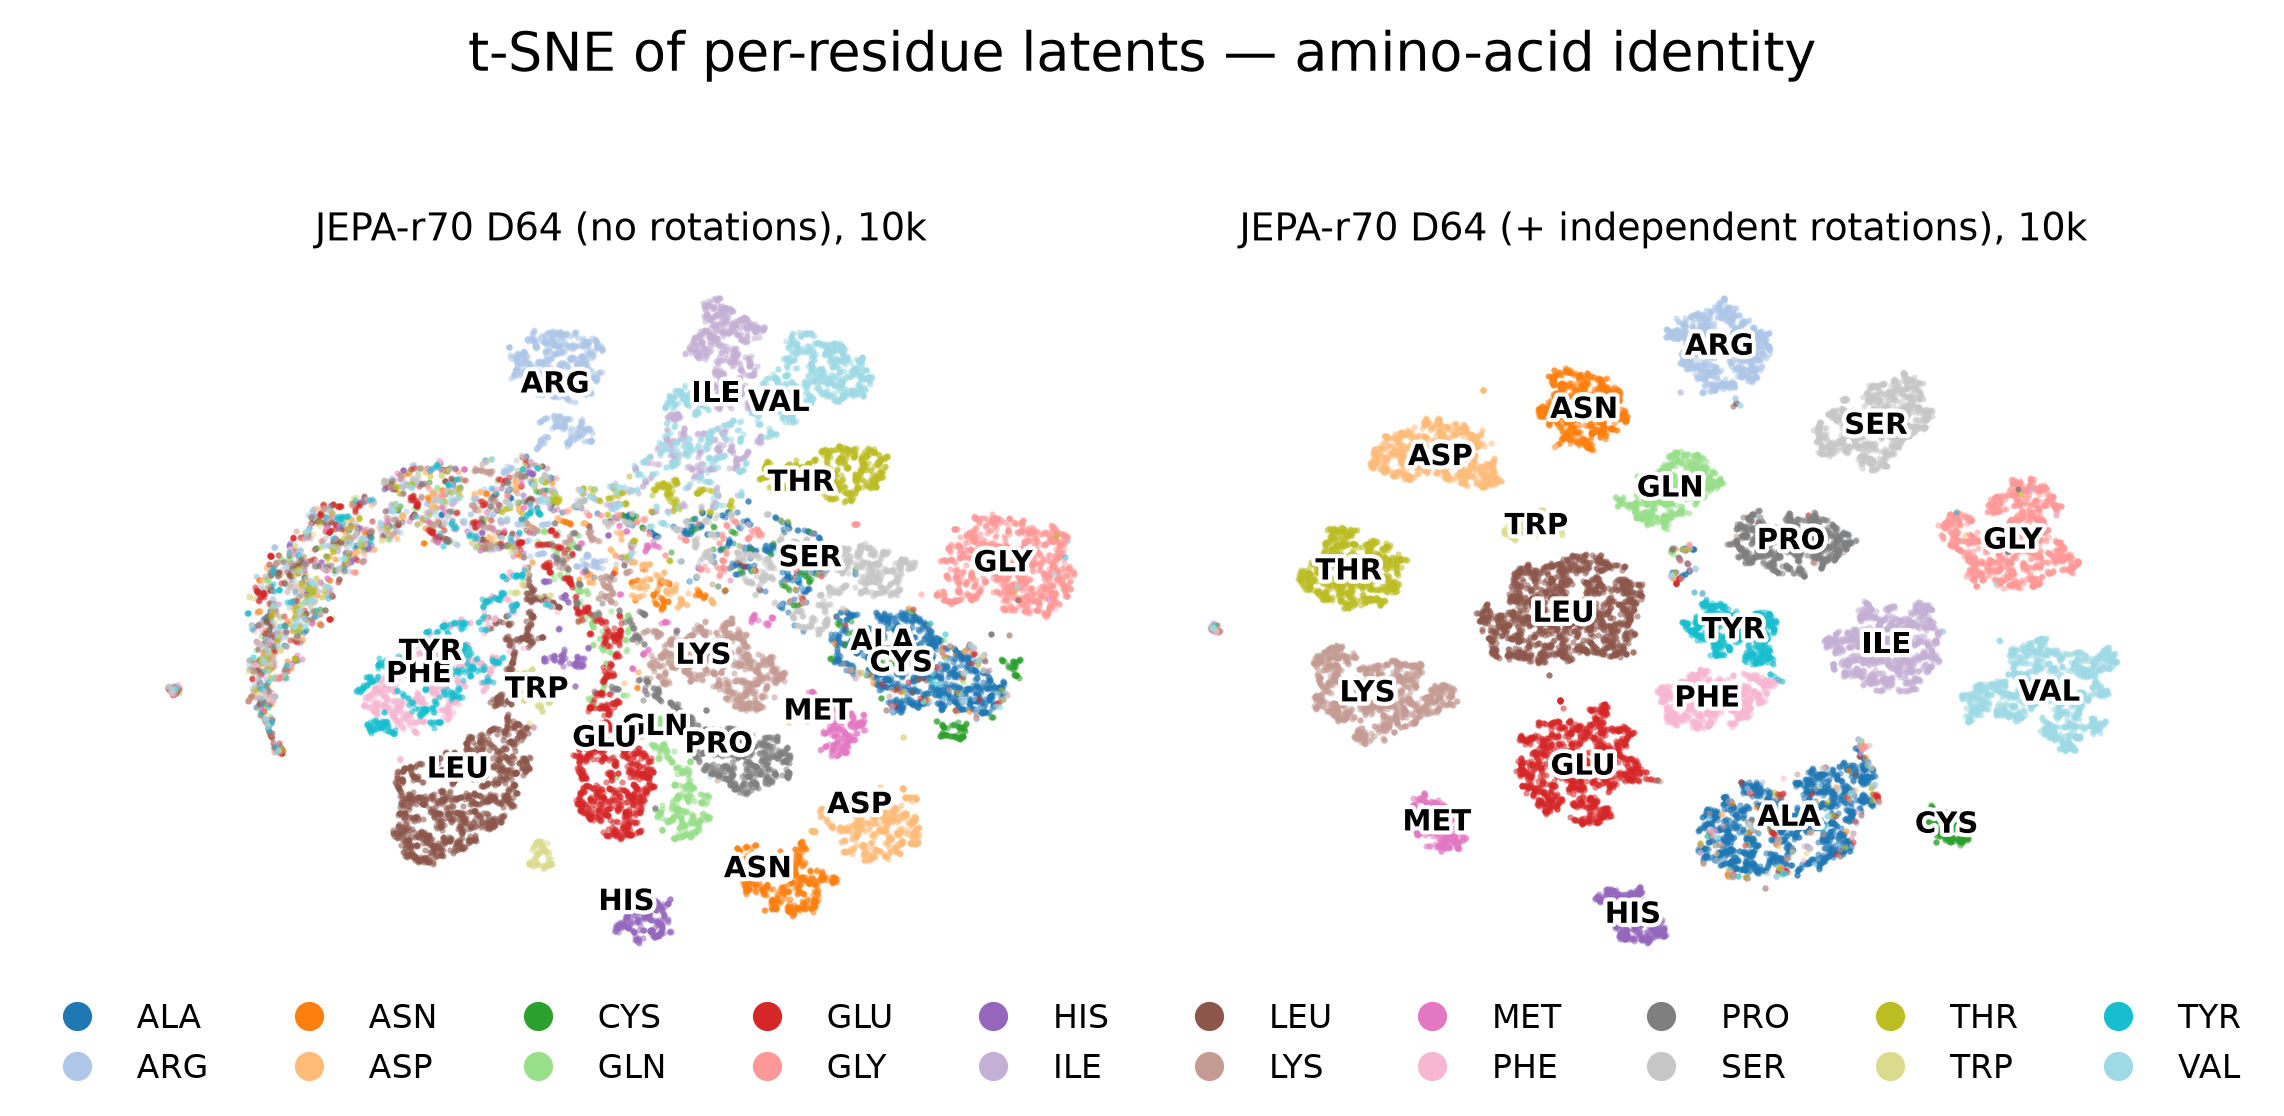
\includegraphics[width=0.88\linewidth]{figures/results/tsne_aa20_jepa-r70-d64-no-rotation-v-rotation_labels-on-clusters.png}
\caption{Matched 10k 64D JEPA rotation diagnostic, with 70\% random masking and points coloured by amino-acid identity. The existing workshop plot uses the same 15,000 sampled residues and visualisation settings in both panels. Cluster separation is qualitative t-SNE evidence, not a quantitative test of rotation invariance or downstream transfer.}
\label{fig:results-rotation-64d-10k}
\end{figure}
\clearpage
\section{Supporting Layerwise Evaluation}
\label{app:layerwise-supporting}
\label{app:jepa-r70-layerwise}
The matched JEPA random-70 evaluation is complete at all three hidden blocks for BindInt, BindBio, BindShake, CatInt and CatBio.
Across these nine task/split scores, block 6 exceeds the final 8D latent in both model families; it is the strongest of the four readouts on 7/9 canonical LeJEPA scores and 5/9 JEPA scores (Tables~\ref{tab:results-layer-stb} and~\ref{tab:results-layer-stb-jepa-r70}).
This recurrence indicates that the middle-layer advantage is not unique to the canonical LeJEPA objective, although the JEPA comparison currently covers only this five-task subset.

\begin{table}[p]
\centering
\resultstableformat
\setlength{\tabcolsep}{2pt}
\renewcommand{\arraystretch}{0.92}
\caption{Completed layerwise STB for JEPA with 70\% random masking, using raw/online weights at 100k and full-context evaluation. Hidden-block outputs are 768D and the final latent mean is 8D. Scores are multiplied by 100; bold marks the strongest readout for each task/split.}
\label{tab:results-layer-stb-jepa-r70}
\begin{tabular}{@{}llrrrr@{}}
\toprule
\multirow{2}{*}{Task} & \multirow{2}{*}{Split}
& \multicolumn{4}{c}{JEPA, random 70\%} \\[1.8pt]
& & Block 1 & Block 6 & Block 12 & Final 8D \\
\midrule
\multirow{2}{*}{BindInt}
& Fold & 47.86 & \textbf{48.86} & 48.24 & 47.11 \\
& SF   & 88.24 & \textbf{91.95} & 91.59 & 80.06 \\
\multirow{2}{*}{BindBio}
& Fold & 72.61 & \textbf{73.22} & 72.84 & 65.56 \\
& SF   & 72.93 & \textbf{73.85} & 73.76 & 65.31 \\
BindShake
& Test & 78.23 & 78.13 & \textbf{78.38} & 71.85 \\
\multirow{2}{*}{CatInt}
& Fold & 65.69 & \textbf{65.72} & 65.05 & 56.84 \\
& SF   & 88.00 & 91.79 & \textbf{92.00} & 76.71 \\
\multirow{2}{*}{CatBio}
& Fold & \textbf{80.72} & 80.13 & 78.23 & 71.50 \\
& SF   & 89.81 & 89.62 & \textbf{90.39} & 75.36 \\
\bottomrule
\end{tabular}
\end{table}
\clearpage

\paragraph{LeJEPA linear probes.}
\begin{figure}[htbp]
\centering
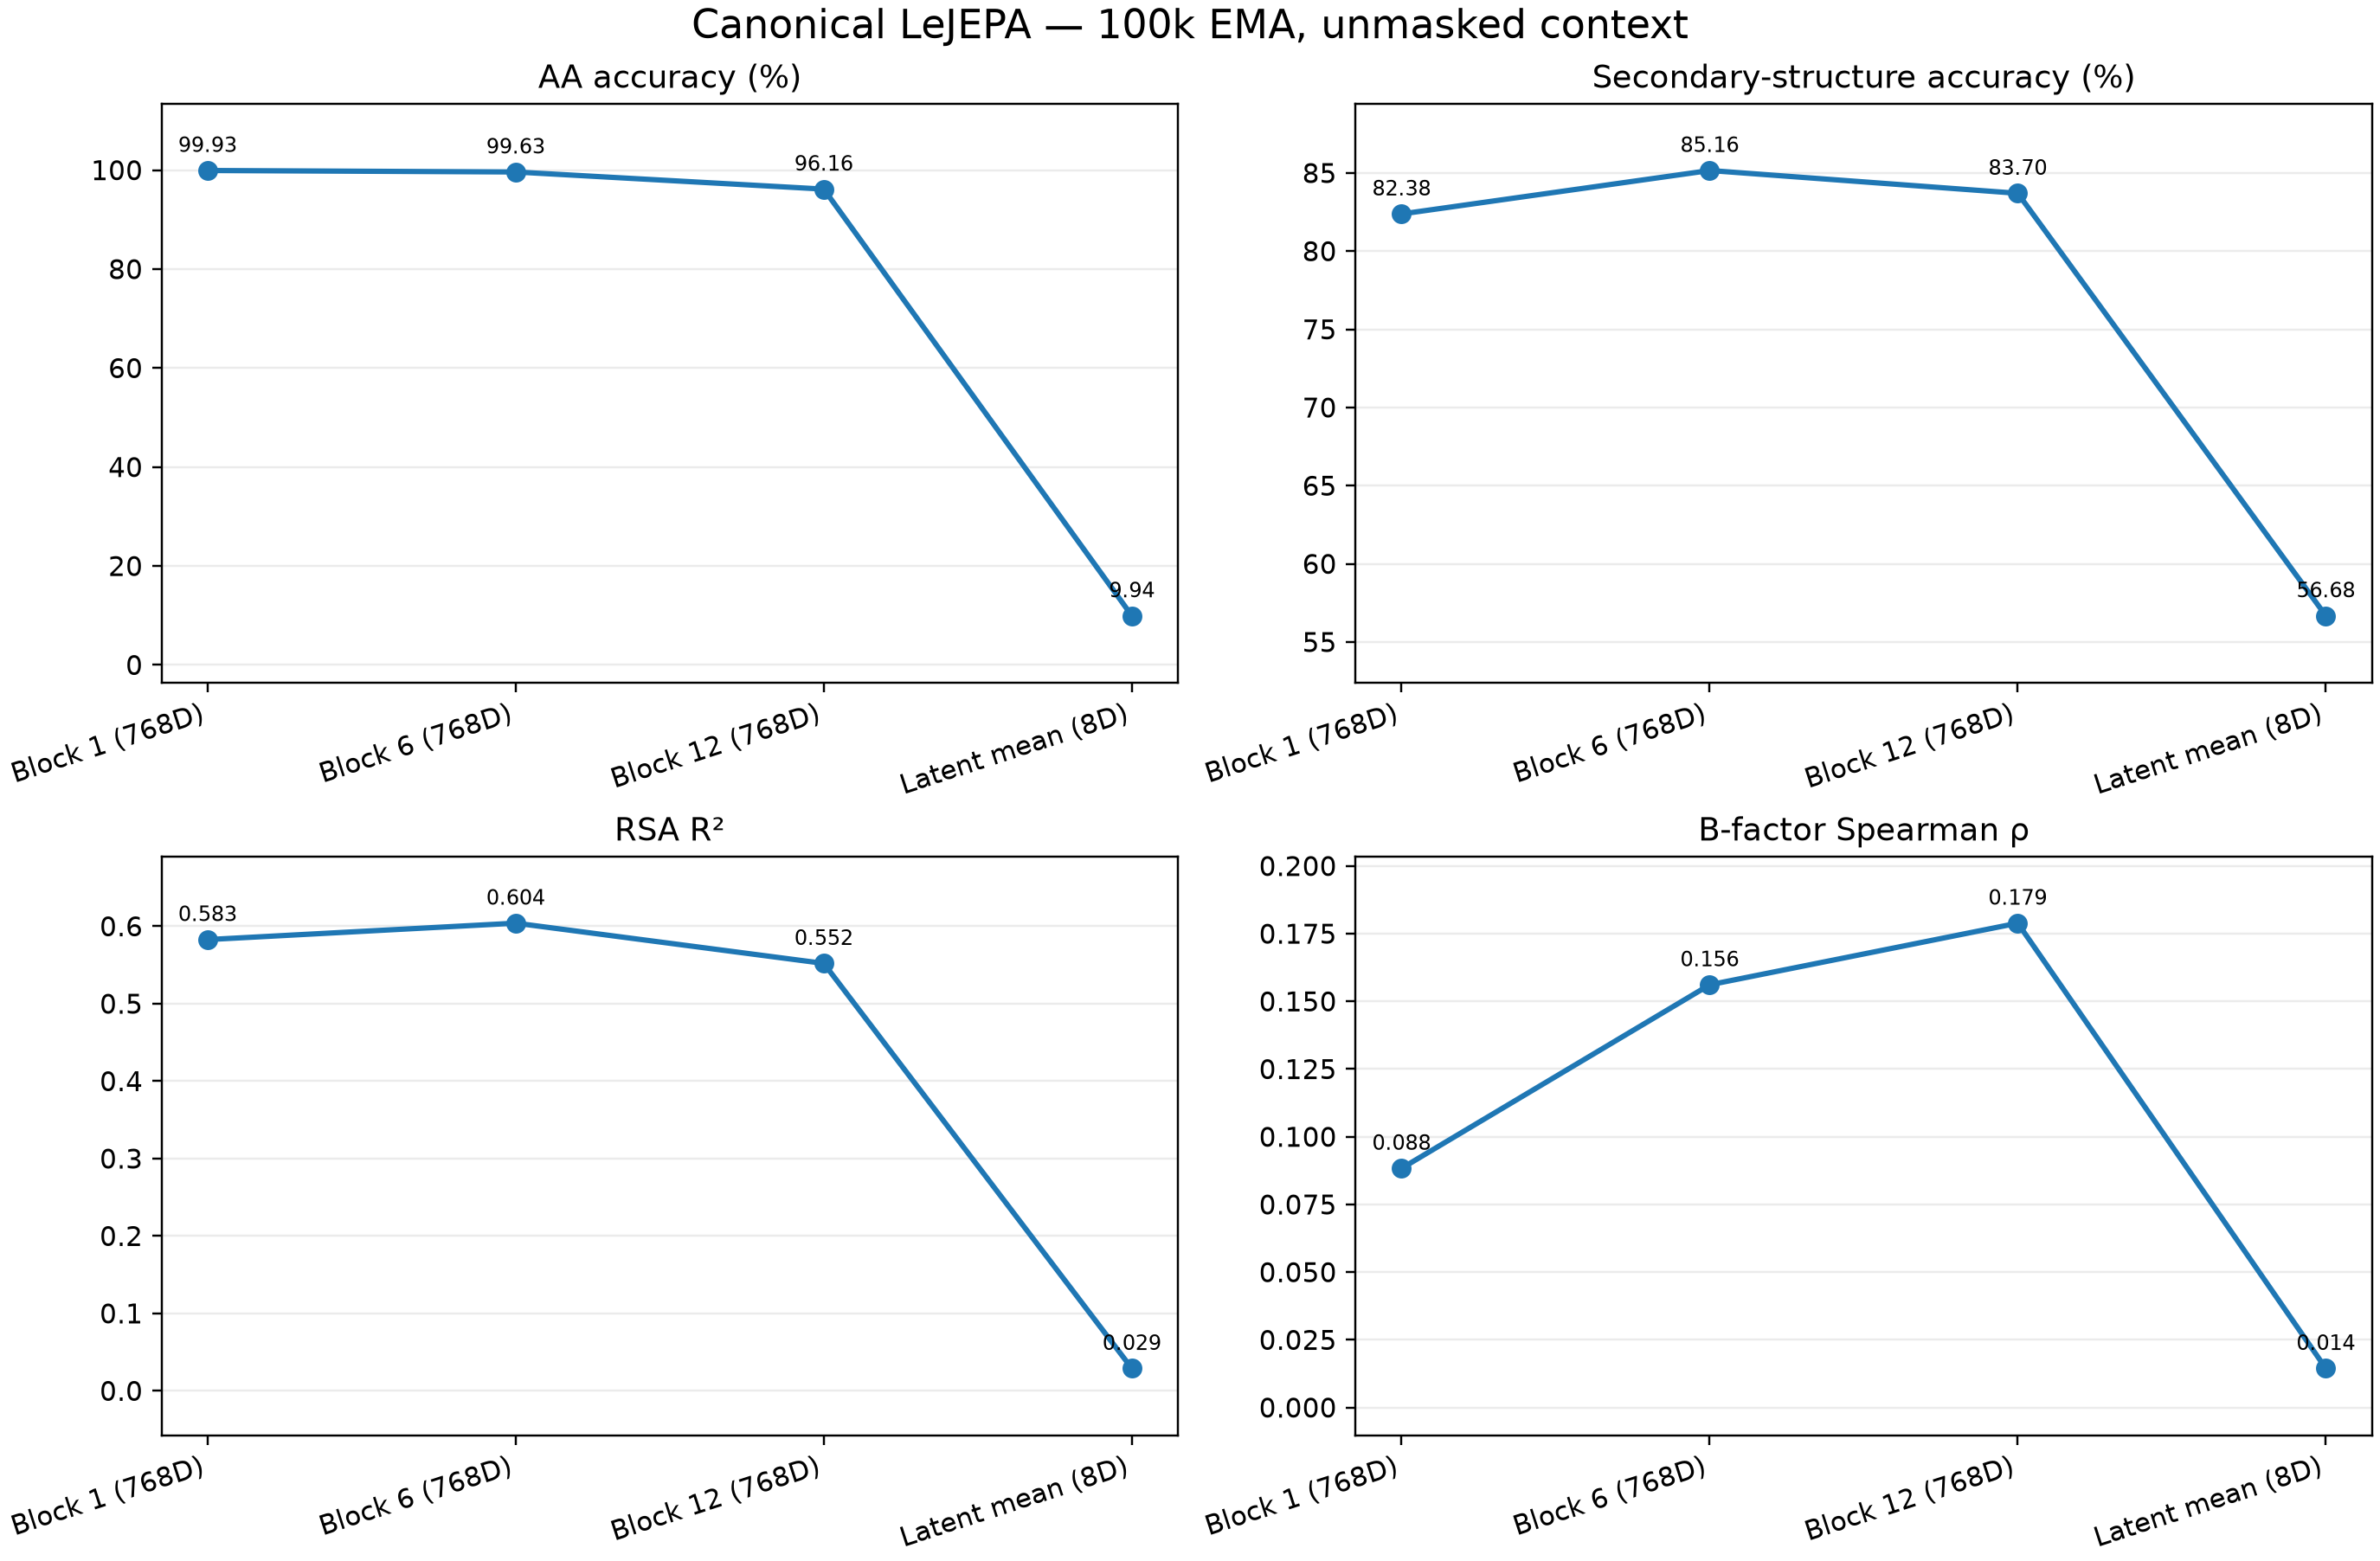
\includegraphics[width=\linewidth]{figures/results/canonical_lejepa_full_context_layerwise_probes.png}
\caption{Full-context linear probes from one uncropped LeJEPA 100k EMA checkpoint. Hidden states are 768D and the final latent mean is 8D. Block-1 SS and block-12 amino-acid/SS fits reported convergence warnings; the highlighted block-6 and latent-mean SS/RSA fits did not. Lines connect different readouts, not a training trajectory.}
\label{fig:results-layer-probes}
\end{figure}
\clearpage
%TC:endignore
